\documentclass[a4paper, 11pt]{article}
\usepackage{geometry}
\usepackage{url}
\usepackage{color}
\usepackage[utf8]{inputenc}
\usepackage[T1]{fontenc}
\usepackage{lmodern}
\usepackage{amsmath,amssymb}
\usepackage{booktabs}
\usepackage{enumitem}
\usepackage{graphicx}
\usepackage[font=small]{caption}
\usepackage{placeins}


\linespread{1}

\geometry{a4paper,top=3cm,left=3cm,right=2.5cm,bottom=2cm}

\usepackage{hyperref}
\hypersetup{colorlinks,linkcolor=blue,citecolor=blue}

\setlist{itemsep=1pt,topsep=3pt}
\setlist[itemize,2]{label=$\circ$}

\newcommand{\feat}[1]{\texttt{#1}}


\title{\textbf{Laboratory assignment} \\[1ex] \large \textbf{Component} (2) -- Data analysis}

\author{\textbf{Authors:} Ștefan-Lucian Grămadă\\ \textbf{Group:} ICA1}

\begin{document}

\maketitle

\section{Analysis of the features used in learning}

\subsection{Correlation}


\begin{table}[htbp]
\centering
\caption{Pairs of features by strength of correlation.}
\label{tab:correlation}
\begin{tabular}{lrrrr}
\toprule
 & \multicolumn{2}{c}{Pearson} & \multicolumn{2}{c}{Spearman} \\
\cmidrule(lr){2-3} \cmidrule(lr){4-5}
Condition & pairs & \% & pairs & \% \\
\midrule
$|r| \geq 0.5$  & 64\,879 & 41.3 & 85\,093 & 54.2 \\
$|r| \geq 0.8$  & 22\,815 & 14.5 & 61\,248 & 39.0 \\
$|r| \geq 0.9$  & 8\,093  & 5.2  & 27\,130 & 17.3 \\
$|r| \geq 0.95$ & 2\,219  & 1.4  & 4\,249  & 2.7 \\
$|r| \geq 0.99$ & 207     & 0.1  & 492     & 0.3 \\
$|r| < 0.2$     & 51\,275 & 32.6 & 40\,444 & 25.7 \\
\bottomrule
\end{tabular}
\end{table}

\begin{table}[htbp]
\centering
\caption{Pairs of features by band of correlation.}
\label{tab:correlationbands}
\begin{tabular}{lrrrr}
\toprule
 & \multicolumn{2}{c}{Pearson} & \multicolumn{2}{c}{Spearman} \\
\cmidrule(lr){2-3} \cmidrule(lr){4-5}
Band & pairs & \% & pairs & \% \\
\midrule
$0 \leq |r| < 0.2$   & 51\,275 & 32.6 & 40\,444 & 25.7 \\
$0.2 \leq |r| < 0.5$ & 40\,926 & 26.1 & 31\,543 & 20.1 \\
$0.5 \leq |r| < 0.8$ & 42\,064 & 26.8 & 23\,845 & 15.2 \\
$0.8 \leq |r| < 0.9$ & 14\,722 & 9.4  & 34\,118 & 21.7 \\
$0.9 \leq |r| \leq 1$ & 8\,093 & 5.2  & 27\,130 & 17.3 \\
\bottomrule
\end{tabular}
\end{table}

\begin{table}[htbp]
\centering
\caption{Notable pairs of distinct features.}
\label{tab:pairs}
\footnotesize
\begin{tabular}{llrr}
\toprule
Feature 1 & Feature 2 & Pearson & Spearman \\
\midrule
\texttt{tBodyAccJerk-energy()-X} & \texttt{fBodyAccJerk-energy()-X} & 1.000 & 1.000 \\
\texttt{tGravityAcc-arCoeff()-Z,1} & \texttt{tGravityAcc-arCoeff()-Z,2} & $-0.995$ & $-0.995$ \\
\texttt{tGravityAcc-mean()-Z} & \texttt{angle(Z,gravityMean)} & $-0.995$ & $-1.000$ \\
\texttt{fBodyGyro-bandsEnergy()-1,8\_2} & \texttt{fBodyGyro-bandsEnergy()-17,24\_2} & 0.273 & 0.881 \\
\bottomrule
\end{tabular}
\end{table}

\begin{table}[htbp]
\centering
\caption{Groups of identical features.}
\label{tab:identical}
\footnotesize
\begin{tabular}{rp{0.85\textwidth}}
\toprule
Group & Features \\
\midrule
1 & \feat{tBodyAccMag-mean()}, \feat{tBodyAccMag-sma()}, \feat{tGravityAccMag-mean()}, \feat{tGravityAccMag-sma()} \\
2 & \feat{tBodyAccMag-std()}, \feat{tGravityAccMag-std()} \\
3 & \feat{tBodyAccMag-mad()}, \feat{tGravityAccMag-mad()} \\
4 & \feat{tBodyAccMag-max()}, \feat{tGravityAccMag-max()} \\
5 & \feat{tBodyAccMag-min()}, \feat{tGravityAccMag-min()} \\
6 & \feat{tBodyAccMag-energy()}, \feat{tGravityAccMag-energy()} \\
7 & \feat{tBodyAccMag-iqr()}, \feat{tGravityAccMag-iqr()} \\
8 & \feat{tBodyAccMag-entropy()}, \feat{tGravityAccMag-entropy()} \\
9 & \feat{tBodyAccMag-arCoeff()1}, \feat{tGravityAccMag-arCoeff()1} \\
10 & \feat{tBodyAccMag-arCoeff()2}, \feat{tGravityAccMag-arCoeff()2} \\
11 & \feat{tBodyAccMag-arCoeff()3}, \feat{tGravityAccMag-arCoeff()3} \\
12 & \feat{tBodyAccMag-arCoeff()4}, \feat{tGravityAccMag-arCoeff()4} \\
13 & \feat{tBodyAccJerkMag-mean()}, \feat{tBodyAccJerkMag-sma()} \\
14 & \feat{tBodyGyroMag-mean()}, \feat{tBodyGyroMag-sma()} \\
15 & \feat{tBodyGyroJerkMag-mean()}, \feat{tBodyGyroJerkMag-sma()} \\
16 & \feat{fBodyAccMag-mean()}, \feat{fBodyAccMag-sma()} \\
17 & \feat{fBodyBodyAccJerkMag-mean()}, \feat{fBodyBodyAccJerkMag-sma()} \\
18 & \feat{fBodyBodyGyroMag-mean()}, \feat{fBodyBodyGyroMag-sma()} \\
19 & \feat{fBodyBodyGyroJerkMag-mean()}, \feat{fBodyBodyGyroJerkMag-sma()} \\
\bottomrule
\end{tabular}
\end{table}

\begin{figure}[htbp]
\centering
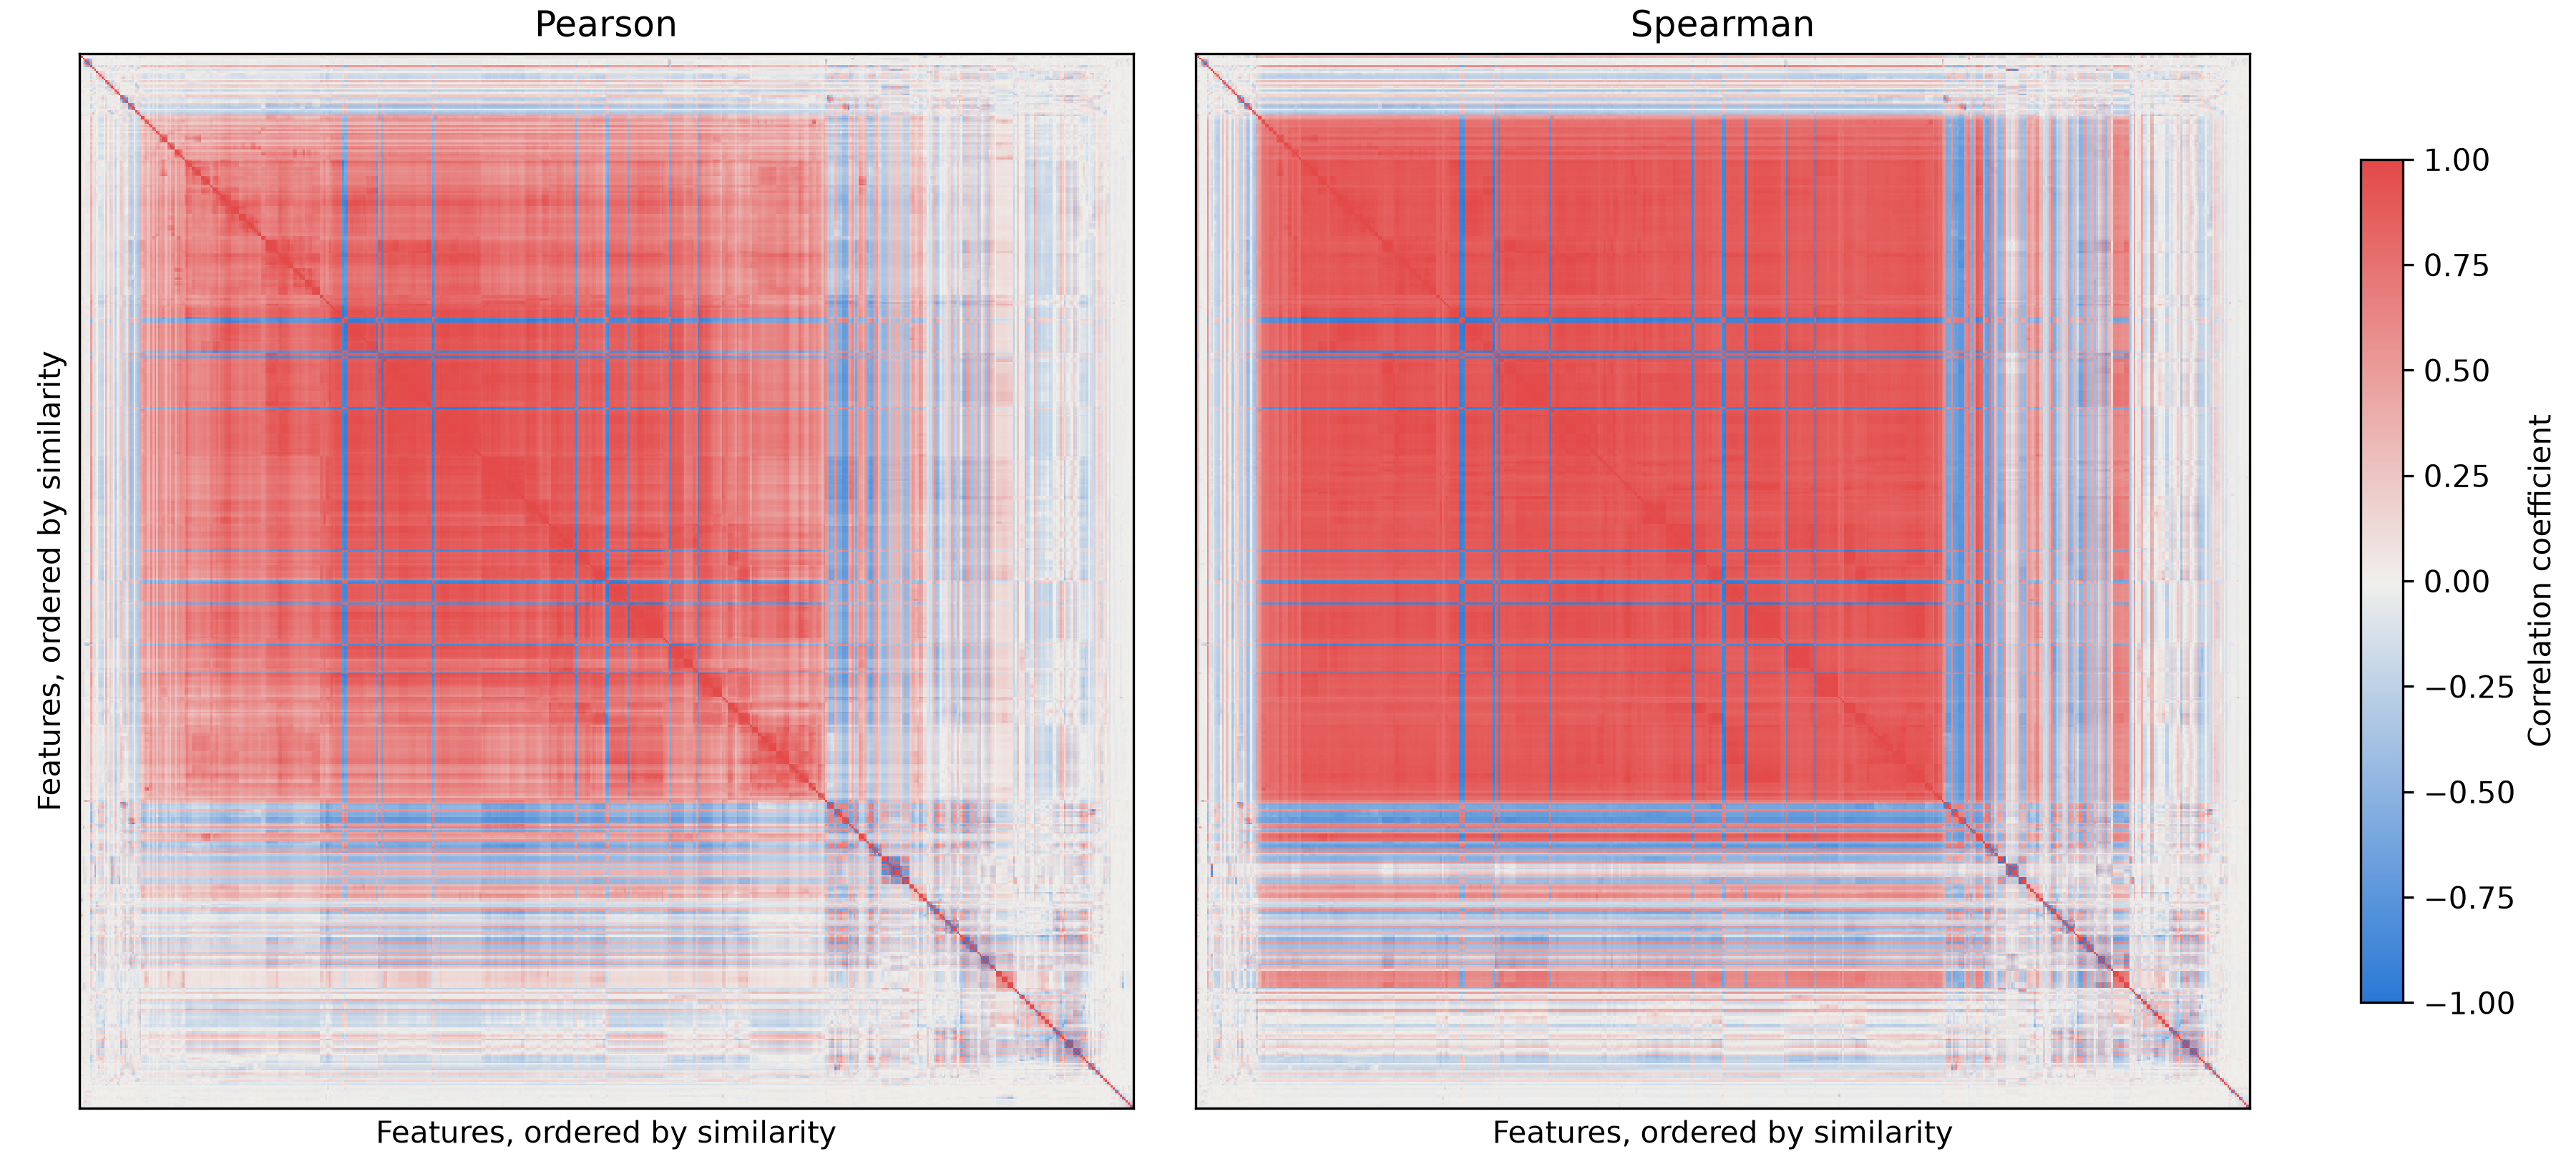
\includegraphics[width=\textwidth]{figures/correlation_heatmaps.png}
\caption{Correlation matrices; features ordered by hierarchical clustering on the Pearson matrix, same order in both panels.}
\label{fig:heatmaps}
\end{figure}

\begin{figure}[htbp]
\centering
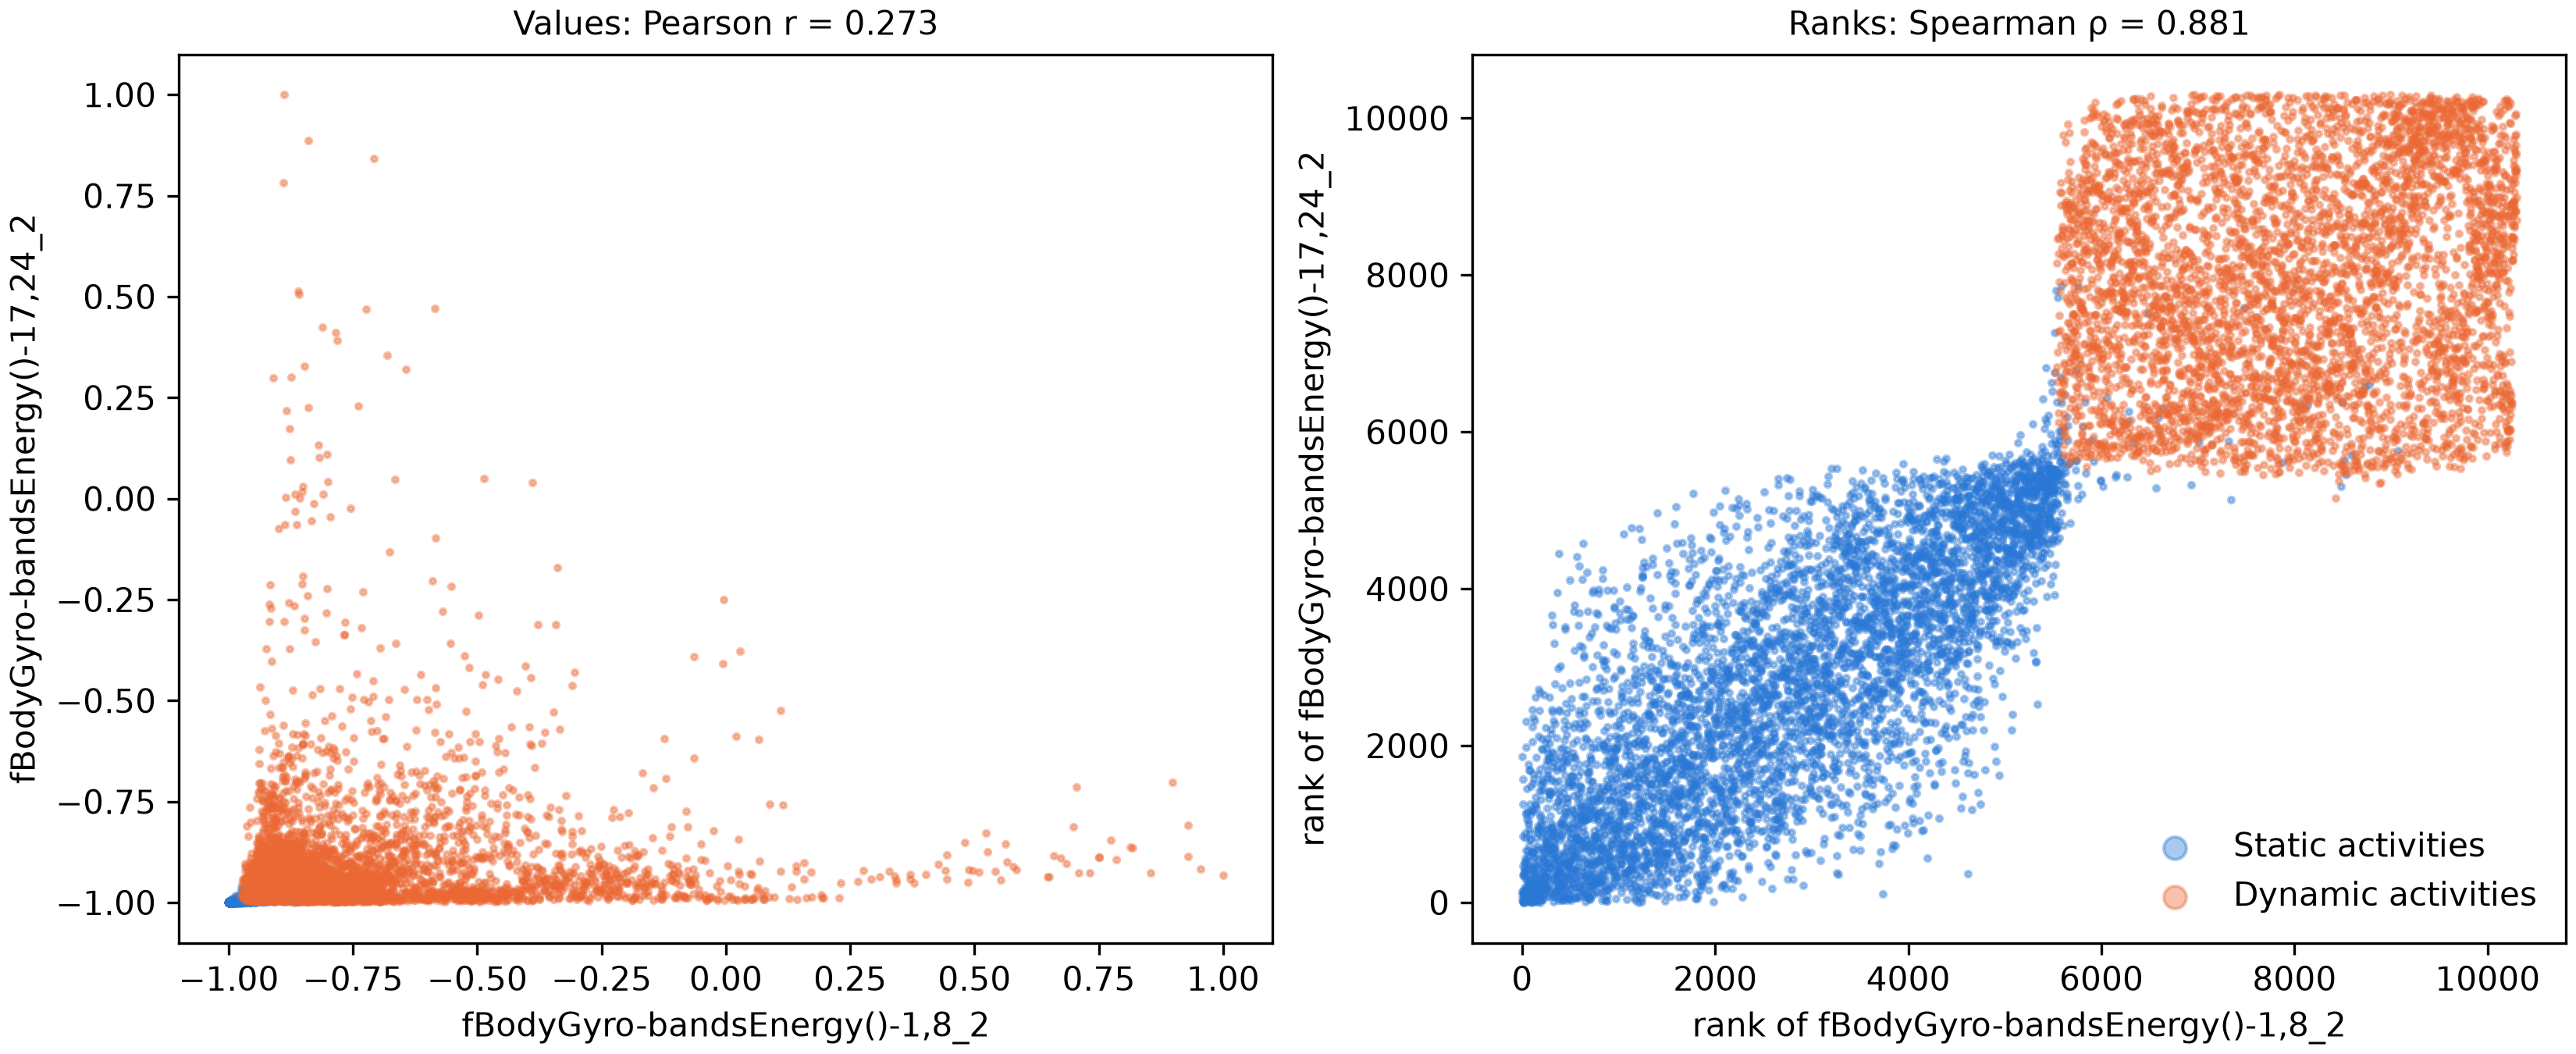
\includegraphics[width=\textwidth]{figures/pearson_vs_spearman.png}
\caption{\feat{fBodyGyro-bandsEnergy()-1,8\_2} vs.\ \feat{fBodyGyro-bandsEnergy()-17,24\_2}: values and ranks, static and dynamic activities.}
\label{fig:pearsonspearman}
\end{figure}

\begin{itemize}
  \item Median $|r|$ = Pearson 0.38, Spearman 0.58.
  \item 19 groups of identical features, 21 redundant copies: \autoref{tab:identical}.
  \item $|\rho| \geq 0.8$ and $|r| < 0.5$: 3\,983 pairs; e.g.\ last row of \autoref{tab:pairs}, \autoref{fig:pearsonspearman}.
  \item \feat{std}, \feat{mad}, \feat{iqr}, \feat{max} of the same signal: strongly correlated. Example, Pearson $r$:
  \begin{itemize}
    \item \feat{tBodyAcc-std()-X} -- \feat{tBodyAcc-mad()-X} = 0.999
    \item \feat{tBodyAcc-std()-X} -- \feat{tBodyAcc-iqr()-X} = 0.981
    \item \feat{tBodyAcc-std()-X} -- \feat{tBodyAcc-max()-X} = 0.981
  \end{itemize}
\end{itemize}

\FloatBarrier
\subsection{Independence}

Pearson's $\chi^2$ test on binned features, Bonferroni-corrected $\alpha = 0.05$.

\begin{table}[htbp]
\centering
\caption{Results of the $\chi^2$ tests.}
\label{tab:independence}
\small
\begin{tabular}{lrr}
\toprule
 & Feature vs.\ activity & Feature vs.\ feature \\
\midrule
Features & 561 & 540 (distinct) \\
Bins & 10 & 5 \\
Tests & 561 & 145\,530 \\
Significance level & $8.9 \times 10^{-5}$ & $3.4 \times 10^{-7}$ \\
Independence rejected & 561 (100\%) & 144\,190 (99.1\%) \\
Cram\'er's $V$: min / median / max & 0.058 / 0.447 / 0.570 & 0.012 / 0.339 / 1.000 \\
$V \geq 0.5$ & 46 (8.2\%) & 47\,393 (32.6\%) \\
$V < 0.1$ & 6 (1.1\%) & 12\,822 (8.8\%) \\
Features with fewer bins (repeated values) & 20 & 17 \\
\bottomrule
\end{tabular}
\end{table}

\begin{table}[htbp]
\centering
\caption{Features most and least dependent on the activity.}
\label{tab:activity}
\footnotesize
\begin{tabular}{lr@{\hspace{2.5em}}lr}
\toprule
Most dependent & $V$ & Least dependent & $V$ \\
\midrule
\texttt{fBodyAcc-bandsEnergy()-1,8\_1} & 0.570 & \texttt{tBodyGyroJerk-arCoeff()-X,4} & 0.058 \\
\texttt{fBodyAcc-bandsEnergy()-1,16\_1} & 0.561 & \texttt{tBodyAccJerkMag-arCoeff()3} & 0.080 \\
\texttt{fBodyAccMag-mad()} & 0.558 & \texttt{tBodyGyroJerk-arCoeff()-Y,4} & 0.081 \\
\texttt{fBodyAcc-std()-X} & 0.558 & \texttt{tBodyGyroJerkMag-arCoeff()3} & 0.083 \\
\texttt{fBodyAccMag-std()} & 0.557 & \texttt{tBodyAcc-arCoeff()-Y,4} & 0.085 \\
\bottomrule
\end{tabular}
\end{table}

\begin{figure}[htbp]
\centering
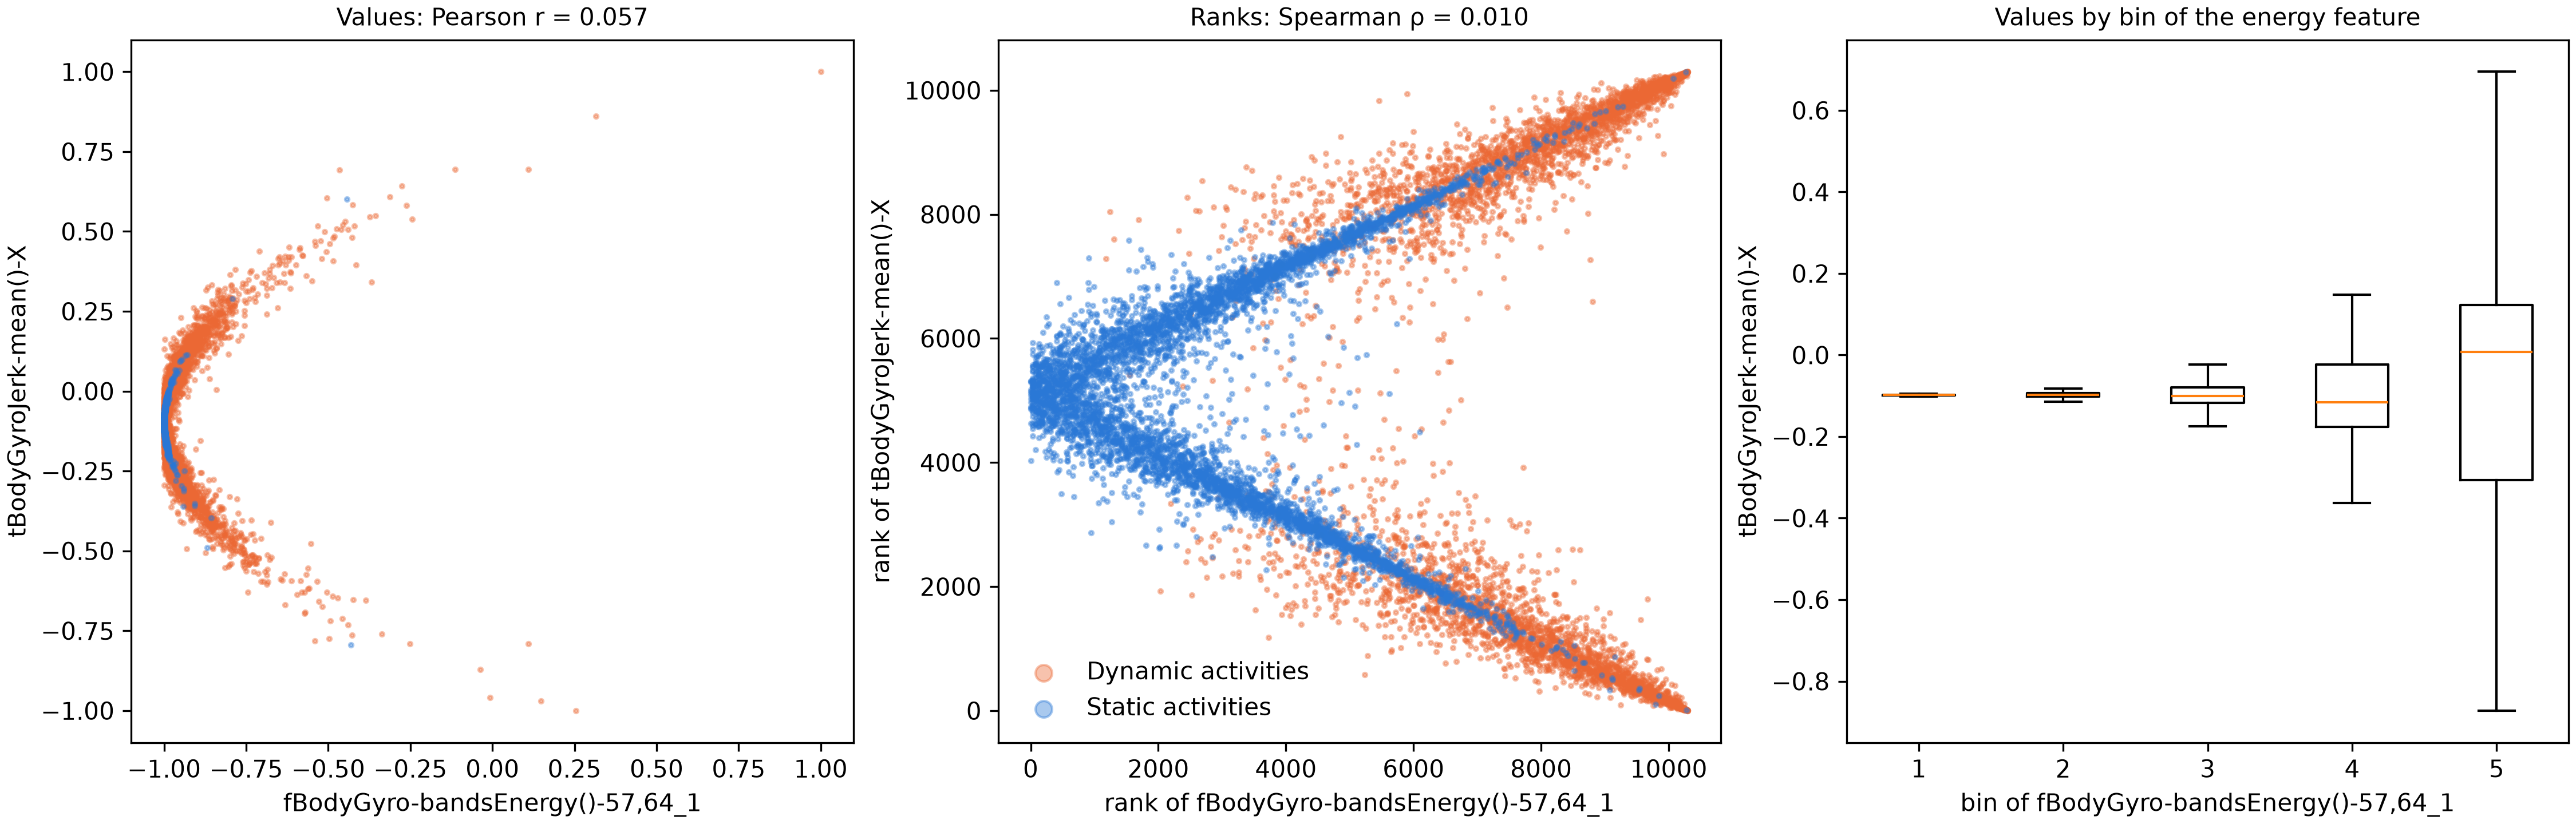
\includegraphics[width=\textwidth]{figures/uncorrelated_dependent.png}
\caption{Uncorrelated but dependent features: values and ranks for static and dynamic activities, and box plots by bin of the energy feature.}
\label{fig:uncorrelated}
\end{figure}

\begin{itemize}
  \item 19\,605 pairs have $|r| < 0.1$ and $|\rho| < 0.1$, but the $\chi^2$ test finds 18\,271 of them dependent, i.e.\ 93.2\%.
  \item Example, \autoref{fig:uncorrelated}:\\ \feat{tBodyGyroJerk-mean()-X} and \feat{fBodyGyro-bandsEnergy()-57,64\_1}: $r = 0.057$, $\rho = 0.010$, $V = 0.580$.
\end{itemize}

\FloatBarrier
\subsection{Feature importance}


\begin{table}[htbp]
\centering
\caption{Top 10 features by each measure.}
\label{tab:importance}
\footnotesize
\begin{tabular}{rlrr}
\toprule
\# & Feature & F & IG (bits) \\
\midrule
\multicolumn{4}{l}{\textit{Ranked by F}} \\
1 & \texttt{fBodyAccJerk-entropy()-X} & 50776 & 0.991 \\
2 & \texttt{tGravityAcc-mean()-X} & 46277 & 0.840 \\
3 & \texttt{tGravityAcc-min()-X} & 44358 & 0.910 \\
4 & \texttt{tGravityAcc-max()-X} & 41203 & 0.777 \\
5 & \texttt{tGravityAcc-energy()-X} & 40416 & 0.840 \\
6 & \texttt{fBodyAccJerk-entropy()-Y} & 37518 & 0.972 \\
7 & \texttt{fBodyBodyAccJerkMag-entropy()} & 32616 & 0.997 \\
8 & \texttt{tBodyAccJerkMag-entropy()} & 32508 & 1.022 \\
9 & \texttt{fBodyAcc-entropy()-X} & 32201 & 1.020 \\
10 & \texttt{tBodyAccJerk-entropy()-X} & 31258 & 0.964 \\
\midrule
\multicolumn{4}{l}{\textit{Ranked by IG}} \\
1 & \texttt{fBodyAcc-bandsEnergy()-1,8\_1} & 7083 & 1.170 \\
2 & \texttt{fBodyAcc-bandsEnergy()-1,16\_1} & 7598 & 1.152 \\
3 & \texttt{fBodyAcc-std()-X} & 22770 & 1.144 \\
4 & \texttt{tBodyAcc-max()-X} & 27862 & 1.142 \\
5 & \texttt{fBodyAcc-bandsEnergy()-1,24\_1} & 7841 & 1.139 \\
6 & \texttt{tBodyAcc-std()-X} & 24559 & 1.135 \\
7 & \texttt{fBodyAcc-energy()-X} & 7875 & 1.135 \\
8 & \texttt{tBodyAcc-energy()-X} & 7756 & 1.134 \\
9 & \texttt{fBodyAcc-max()-X} & 13854 & 1.125 \\
10 & \texttt{tBodyAcc-mad()-X} & 21278 & 1.117 \\
\bottomrule
\end{tabular}
\end{table}

\begin{figure}[htbp]
\centering
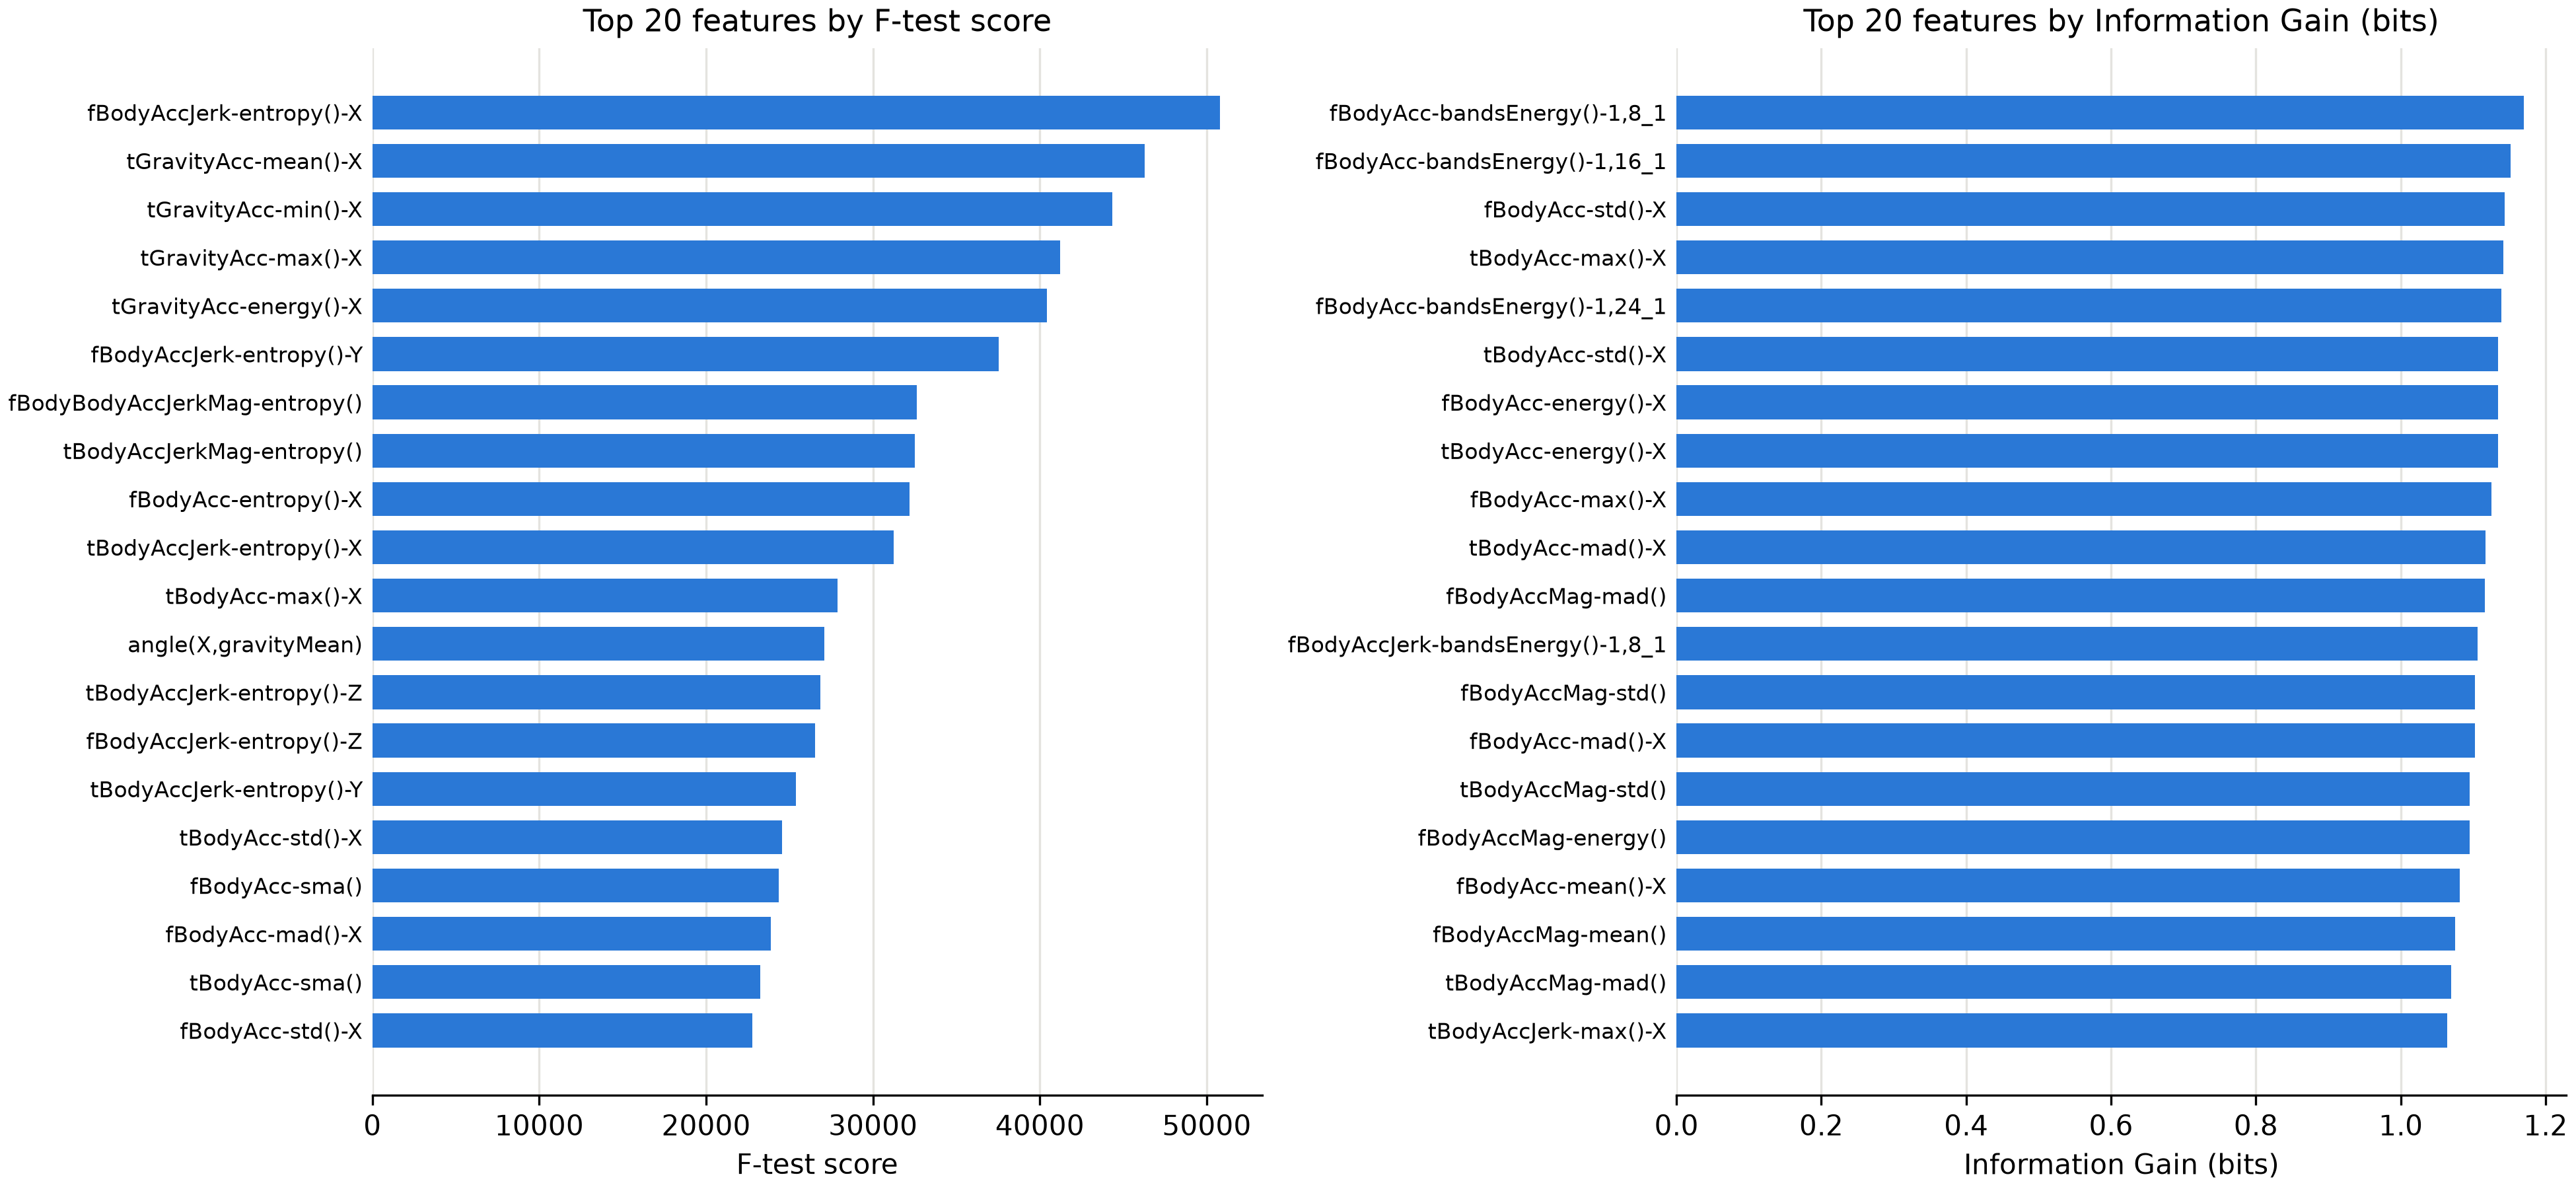
\includegraphics[width=\textwidth]{figures/top_features.png}
\caption{Top 20 features by F-test score and by Information Gain.}
\label{fig:importance}
\end{figure}

\begin{table}[htbp]
\centering
\caption{Median importance by feature family.}
\label{tab:families}
\footnotesize
\begin{tabular}{lrrr@{\hspace{3em}}lrrr}
\toprule
Statistic & $n$ & F & IG & Group & $n$ & F & IG \\
\midrule
\texttt{sma} & 8 & 15857 & 0.991 & \multicolumn{4}{l}{\textit{Sensor}} \\
\texttt{energy} & 32 & 3079 & 0.978 & body acceleration & 286 & 2517 & 0.938 \\
\texttt{mad} & 32 & 9391 & 0.971 & gyroscope & 207 & 1475 & 0.905 \\
\texttt{std} & 32 & 8626 & 0.964 & angle & 7 & 44 & 0.462 \\
\texttt{iqr} & 32 & 7609 & 0.959 & gravity & 40 & 519 & 0.419 \\
\texttt{max} & 32 & 6462 & 0.947 & \multicolumn{4}{l}{\textit{Domain}} \\
\texttt{entropy} & 32 & 13555 & 0.945 & frequency & 285 & 1863 & 0.934 \\
\texttt{bandsEnergy} & 126 & 1634 & 0.939 & time & 248 & 2177 & 0.675 \\
\texttt{mean} & 32 & 6795 & 0.916 & angle & 7 & 44 & 0.462 \\
\texttt{min} & 32 & 3706 & 0.878 & & & & \\
\texttt{angle} & 7 & 44 & 0.462 & & & & \\
\texttt{maxInds} & 13 & 272 & 0.340 & & & & \\
\texttt{meanFreq} & 13 & 473 & 0.234 & & & & \\
\texttt{skewness} & 13 & 268 & 0.184 & & & & \\
\texttt{arCoeff} & 76 & 388 & 0.157 & & & & \\
\texttt{kurtosis} & 13 & 247 & 0.153 & & & & \\
\texttt{correlation} & 15 & 186 & 0.141 & & & & \\
\bottomrule
\end{tabular}
\end{table}

\begin{itemize}
  \item $\max IG = 1.170$ bits, of $H = 2.576$ bits.
  \item Rank correlation F vs.\ IG: 0.789; common features in the two top 20: 4.
  \item Median number of features with $|r| \geq 0.9$ within the same top 20: F 13.5, IG 17.
\end{itemize}

\FloatBarrier
\section{Data statistics}

\begin{table}[htbp]
\centering
\caption{Data set overview: UCI HAR~\cite{anguita2013}, training and test files.}
\label{tab:overview}
\small
\begin{tabular}{lr@{\hspace{3em}}lr}
\toprule
Instances & 10\,299 & Volunteers & 30 \\
Training / test instances & 7\,352 / 2\,947 & Activities & 6 \\
Features & 561 & Missing values & 0 \\
Distinct features & 540 & Repeated rows & 0 \\
\bottomrule
\end{tabular}
\end{table}

\begin{table}[htbp]
\centering
\caption{Instances per activity.}
\label{tab:classes}
\small
\begin{tabular}{lrrrrrr}
\toprule
 & Walking & Upstairs & Downstairs & Sitting & Standing & Laying \\
\midrule
Instances & 1\,722 & 1\,544 & 1\,406 & 1\,777 & 1\,906 & 1\,944 \\
Share (\%) & 16.7 & 15.0 & 13.7 & 17.3 & 18.5 & 18.9 \\
\bottomrule
\end{tabular}
\end{table}

\begin{itemize}
  \item Class balance: largest / smallest class $= 1944 / 1406 = 1.38$.
  \item Instances per volunteer: $\min = 281$, $\max = 409$, $\mathrm{median} = 342.5$.
  \item Instances per volunteer and activity: $\min = 36$, $\max = 95$, $\mathrm{median} = 54.5$; all 30 volunteers performed all 6 activities.
\end{itemize}

\FloatBarrier
\section{Data distribution}

Studied for the 6 features with the highest Information Gain, \autoref{tab:importance}, skipping features with $|r| \geq 0.9$ to an already selected one.

\begin{table}[htbp]
\centering
\caption{Selected features: importance, shape, outliers and training vs.\ test difference.}
\label{tab:distribution}
\footnotesize
\begin{tabular}{lrrrrrr}
\toprule
Feature & IG & F & Skewness & Kurtosis & Outliers (\%) & KS \\
\midrule
\feat{fBodyAcc-bandsEnergy()-1,8\_1} & 1.170 & 7083 & 1.91 & 4.12 & 5.86 & 0.055 \\
\feat{tBodyAcc-max()-X} & 1.142 & 27862 & 0.60 & $-1.16$ & 0.00 & 0.045 \\
\feat{tBodyAccJerk-energy()-X} & 1.036 & 5001 & 1.80 & 4.31 & 3.75 & 0.065 \\
\feat{tBodyGyroJerk-mad()-X} & 1.009 & 9494 & 0.86 & $-0.09$ & 0.24 & 0.065 \\
\feat{fBodyAccJerk-bandsEnergy()-17,32\_3} & 1.007 & 1579 & 4.19 & 33.15 & 8.41 & 0.060 \\
\feat{fBodyAccJerk-bandsEnergy()-17,24\_2} & 0.999 & 2820 & 2.05 & 4.94 & 6.44 & 0.086 \\
\bottomrule
\end{tabular}
\end{table}

\begin{figure}[htbp]
\centering
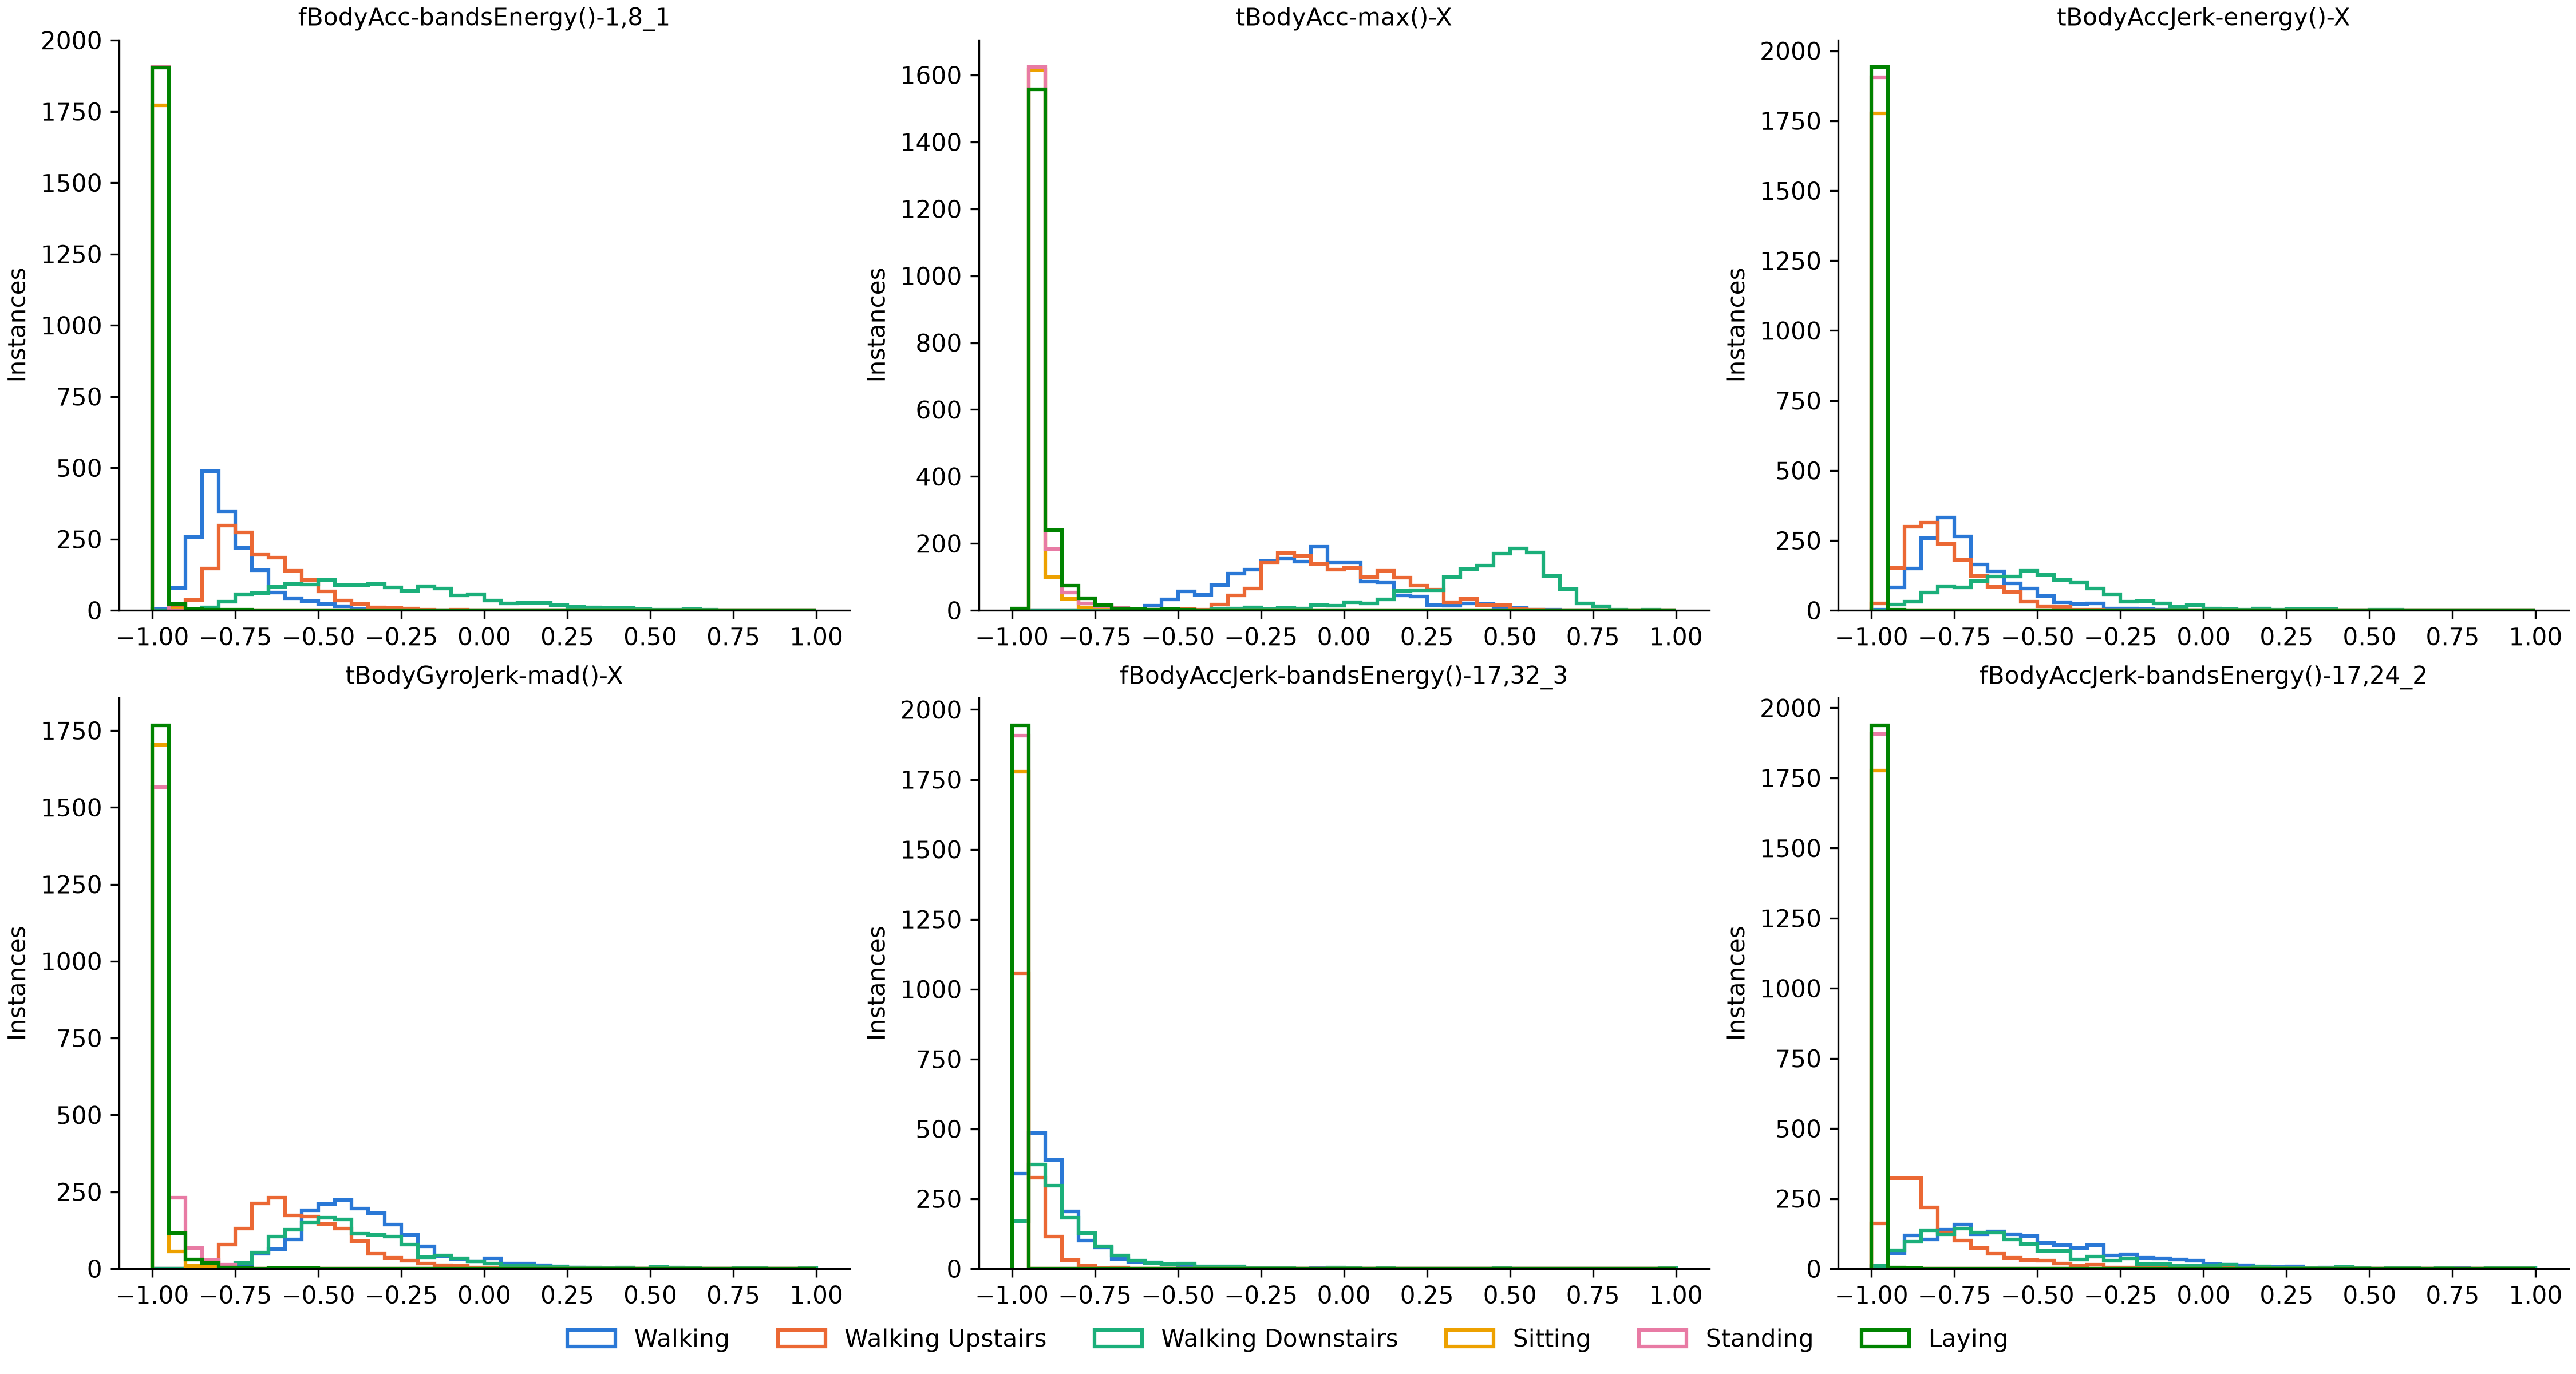
\includegraphics[width=\textwidth]{figures/histograms_by_activity.png}
\caption{Histograms of the selected features, one line per activity.}
\label{fig:histograms}
\end{figure}

\begin{figure}[htbp]
\centering
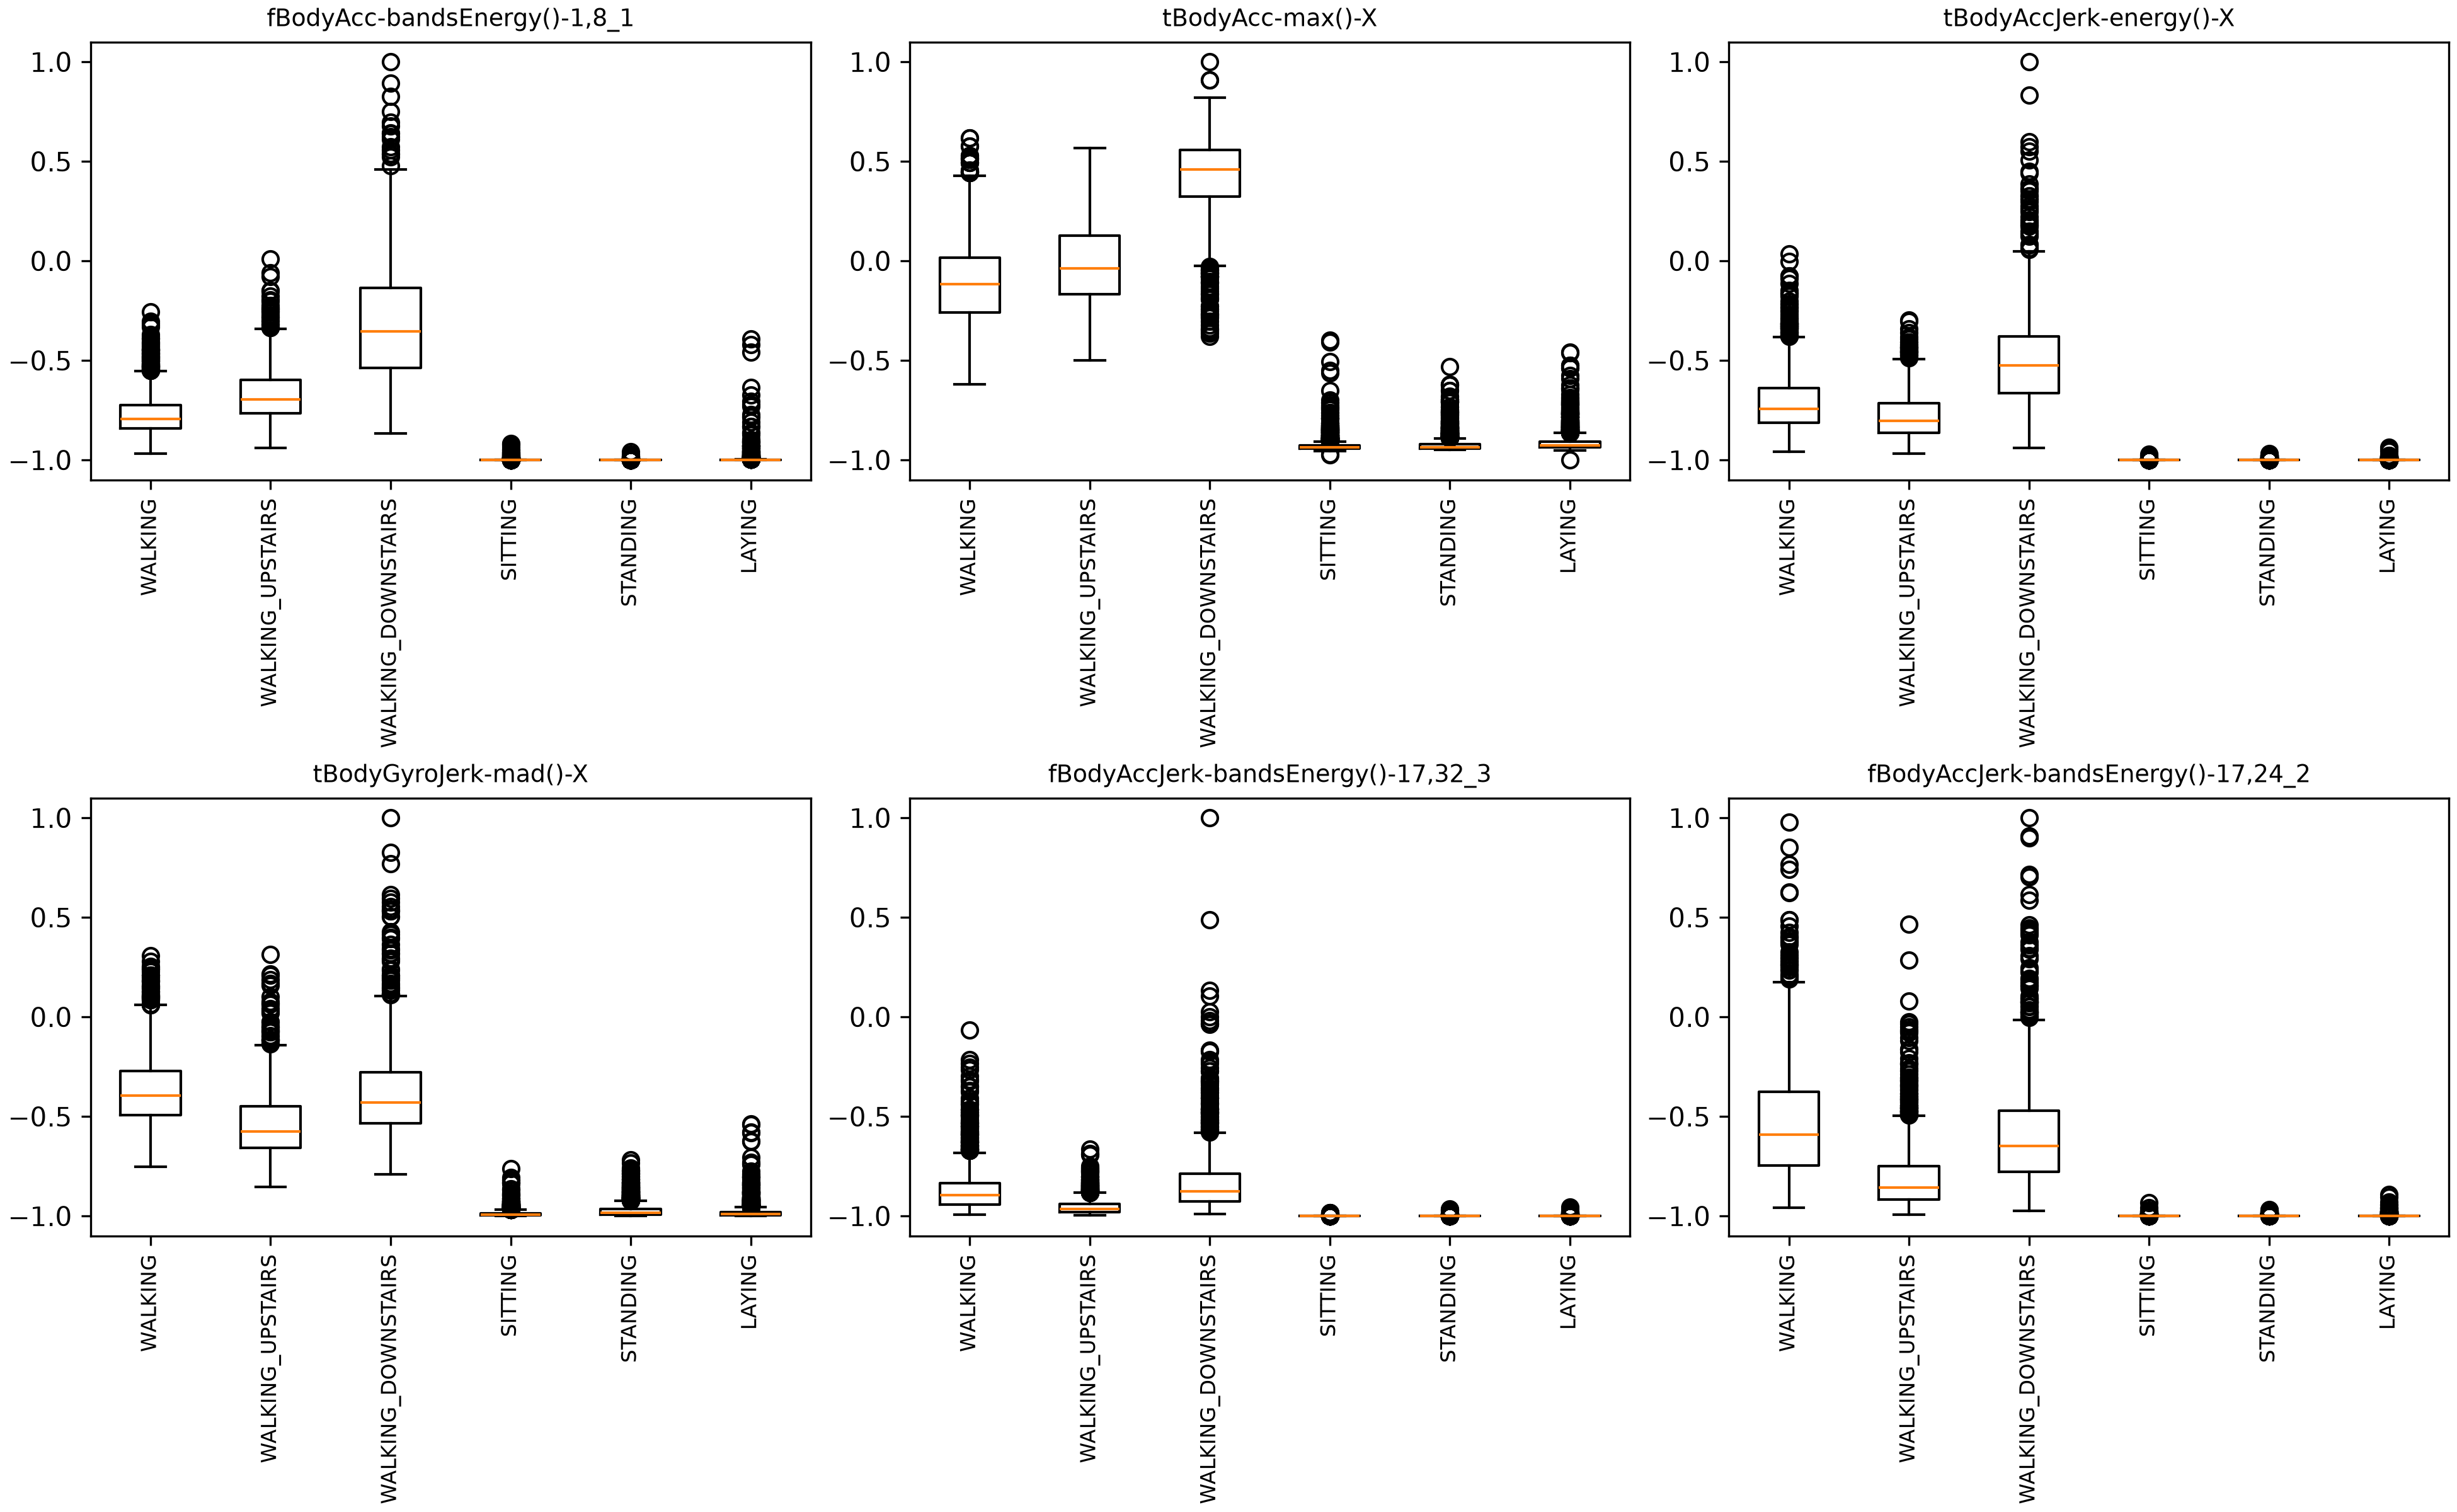
\includegraphics[width=\textwidth]{figures/boxplots_by_activity.png}
\caption{Box plots of the selected features by activity.}
\label{fig:boxplots}
\end{figure}

\begin{itemize}
  \item Static activities: values $\leq -0.8$ for $97.5$--$100\%$ of instances, for all 6 features.
  \item Dynamic activities: spread over $[-1, 1]$; highest values for walking downstairs, e.g.\ \feat{tBodyAcc-max()-X}: $\mathrm{median} = 0.459$.
  \item All 6 features right-skewed: $\mathrm{skewness} \in [0.60, 4.19]$; $\mathrm{outliers} \in [0, 8.4]\%$, mainly in the tails.
  \item Training vs.\ test: Kolmogorov--Smirnov statistic $\leq 0.086$.
\end{itemize}

\FloatBarrier
\section{Data visualization and interpretation}

\begin{figure}[htbp]
\centering
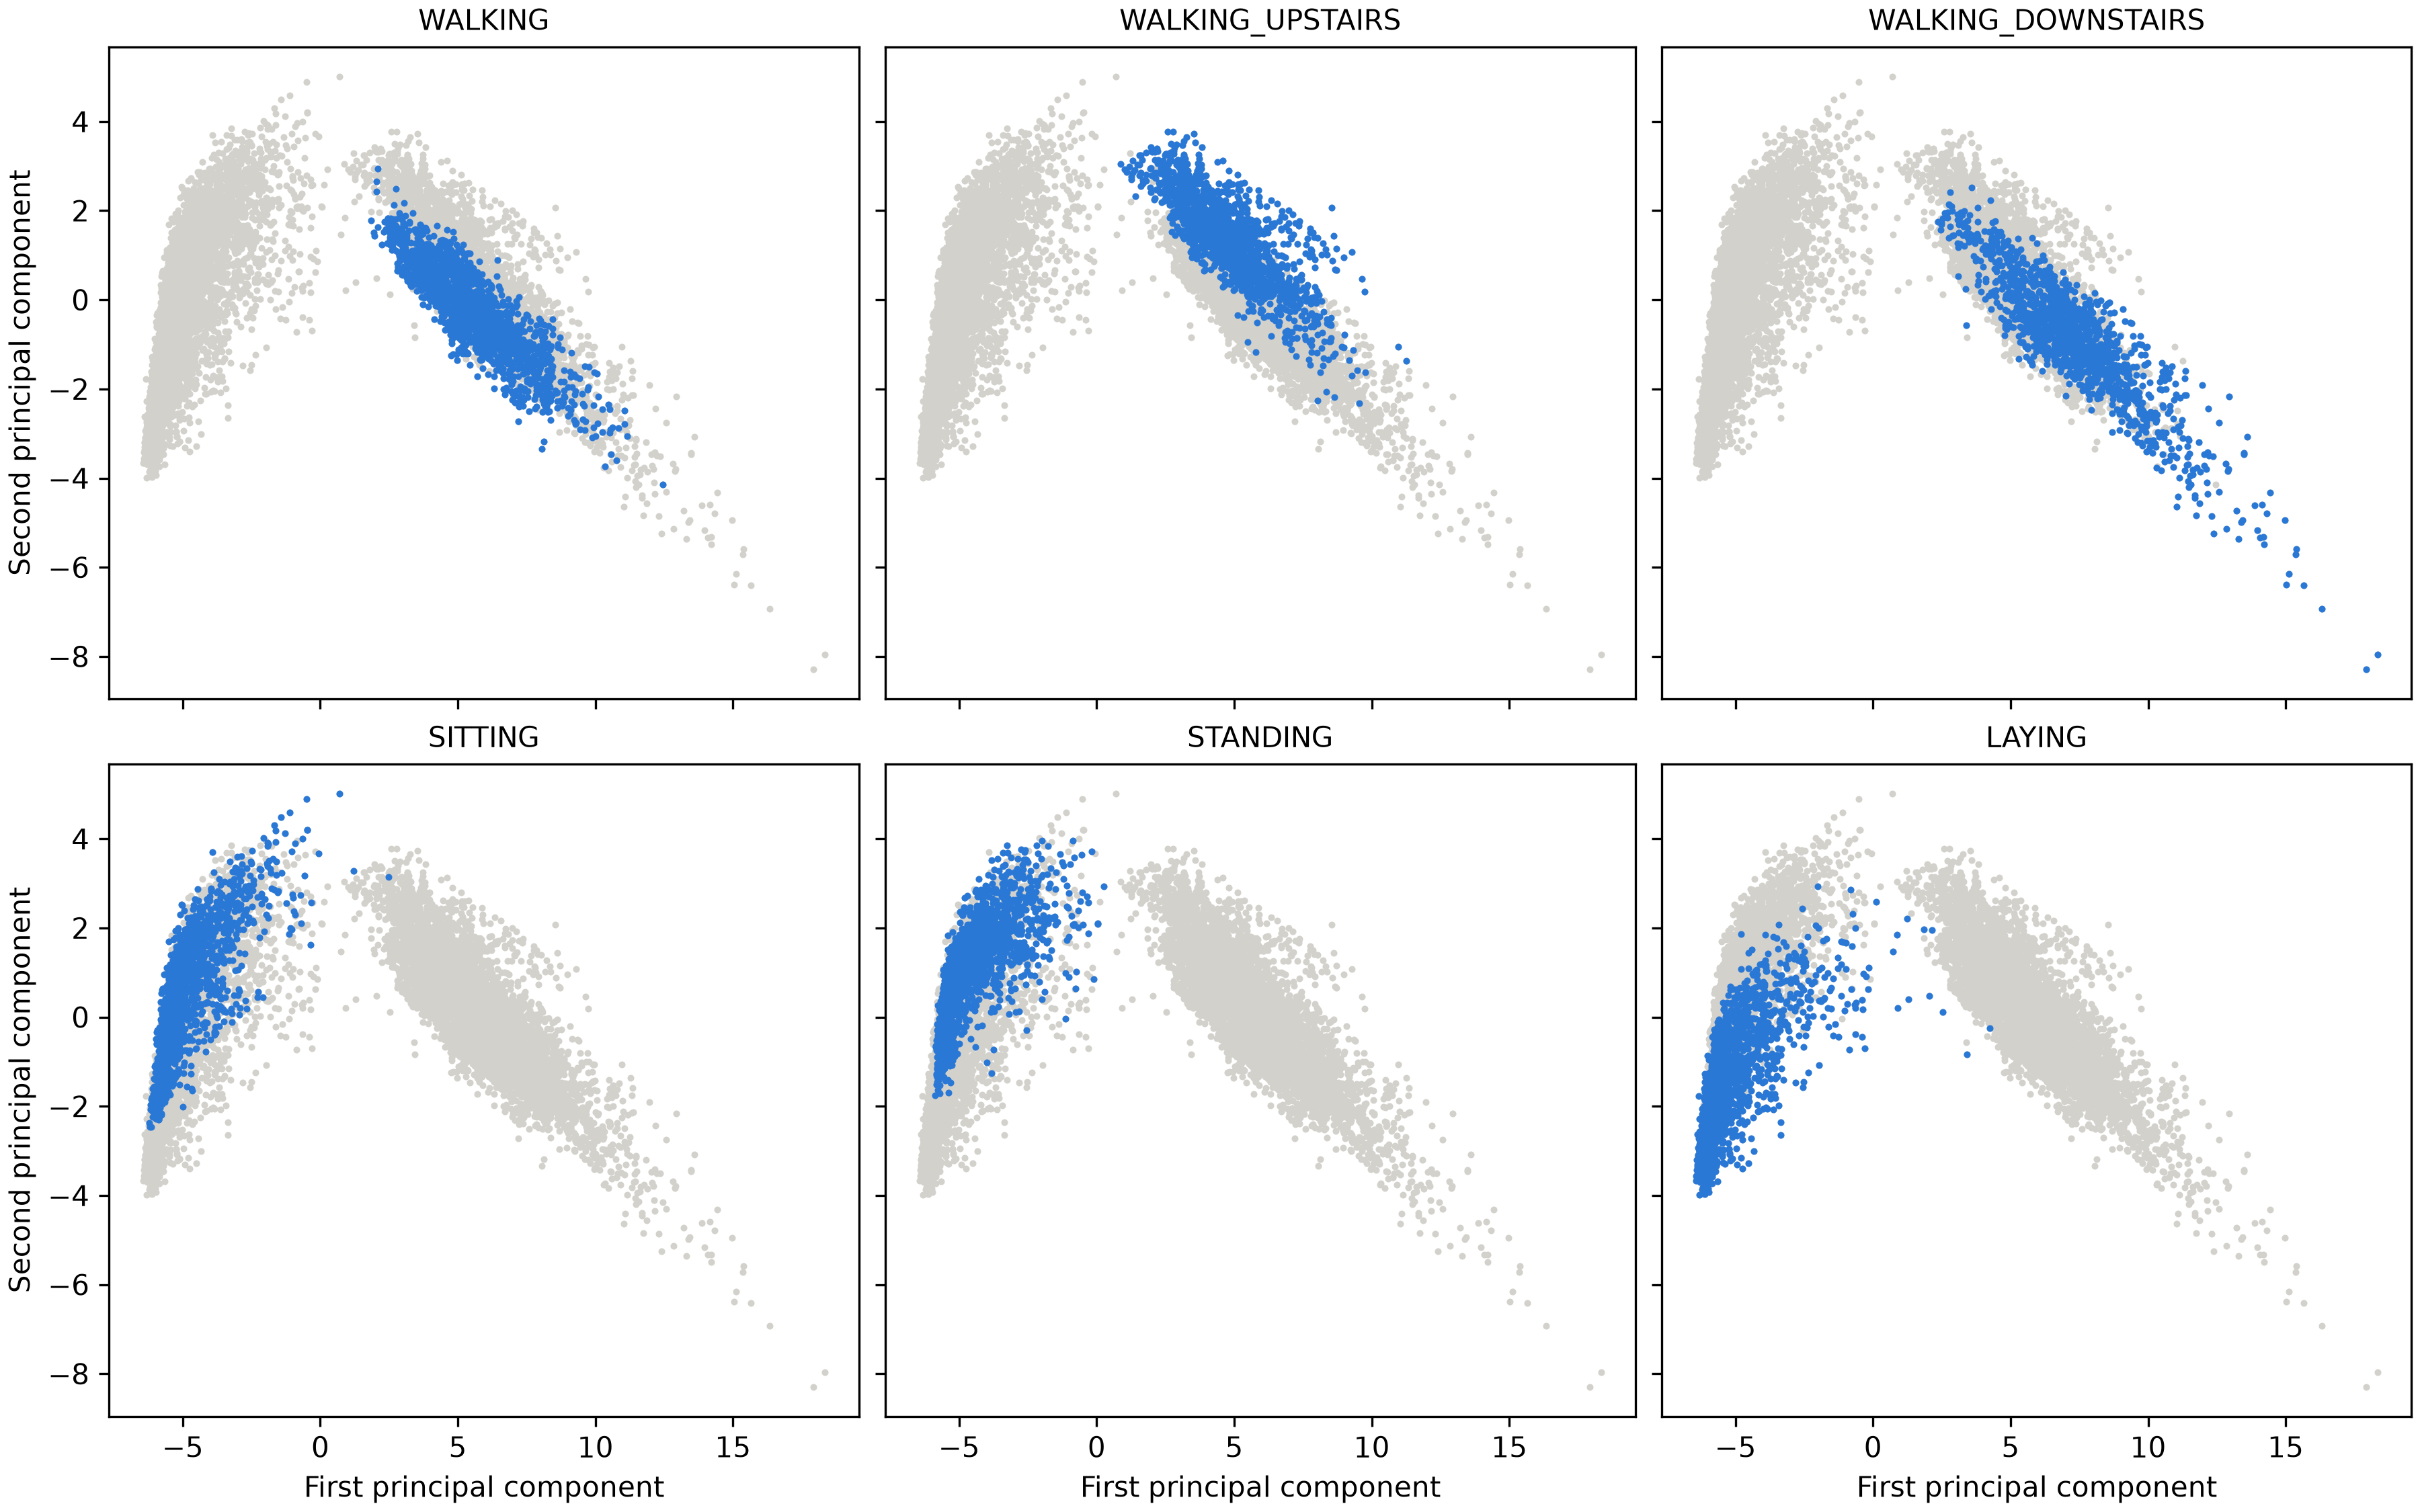
\includegraphics[width=0.85\textwidth]{figures/pca.png}
\caption{PCA projection of the 540 distinct features; explained variance: PC1 60.8\%, PC2 4.8\%. Blue: the activity of the panel; grey: all instances.}
\label{fig:pca}
\end{figure}

\begin{figure}[htbp]
\centering
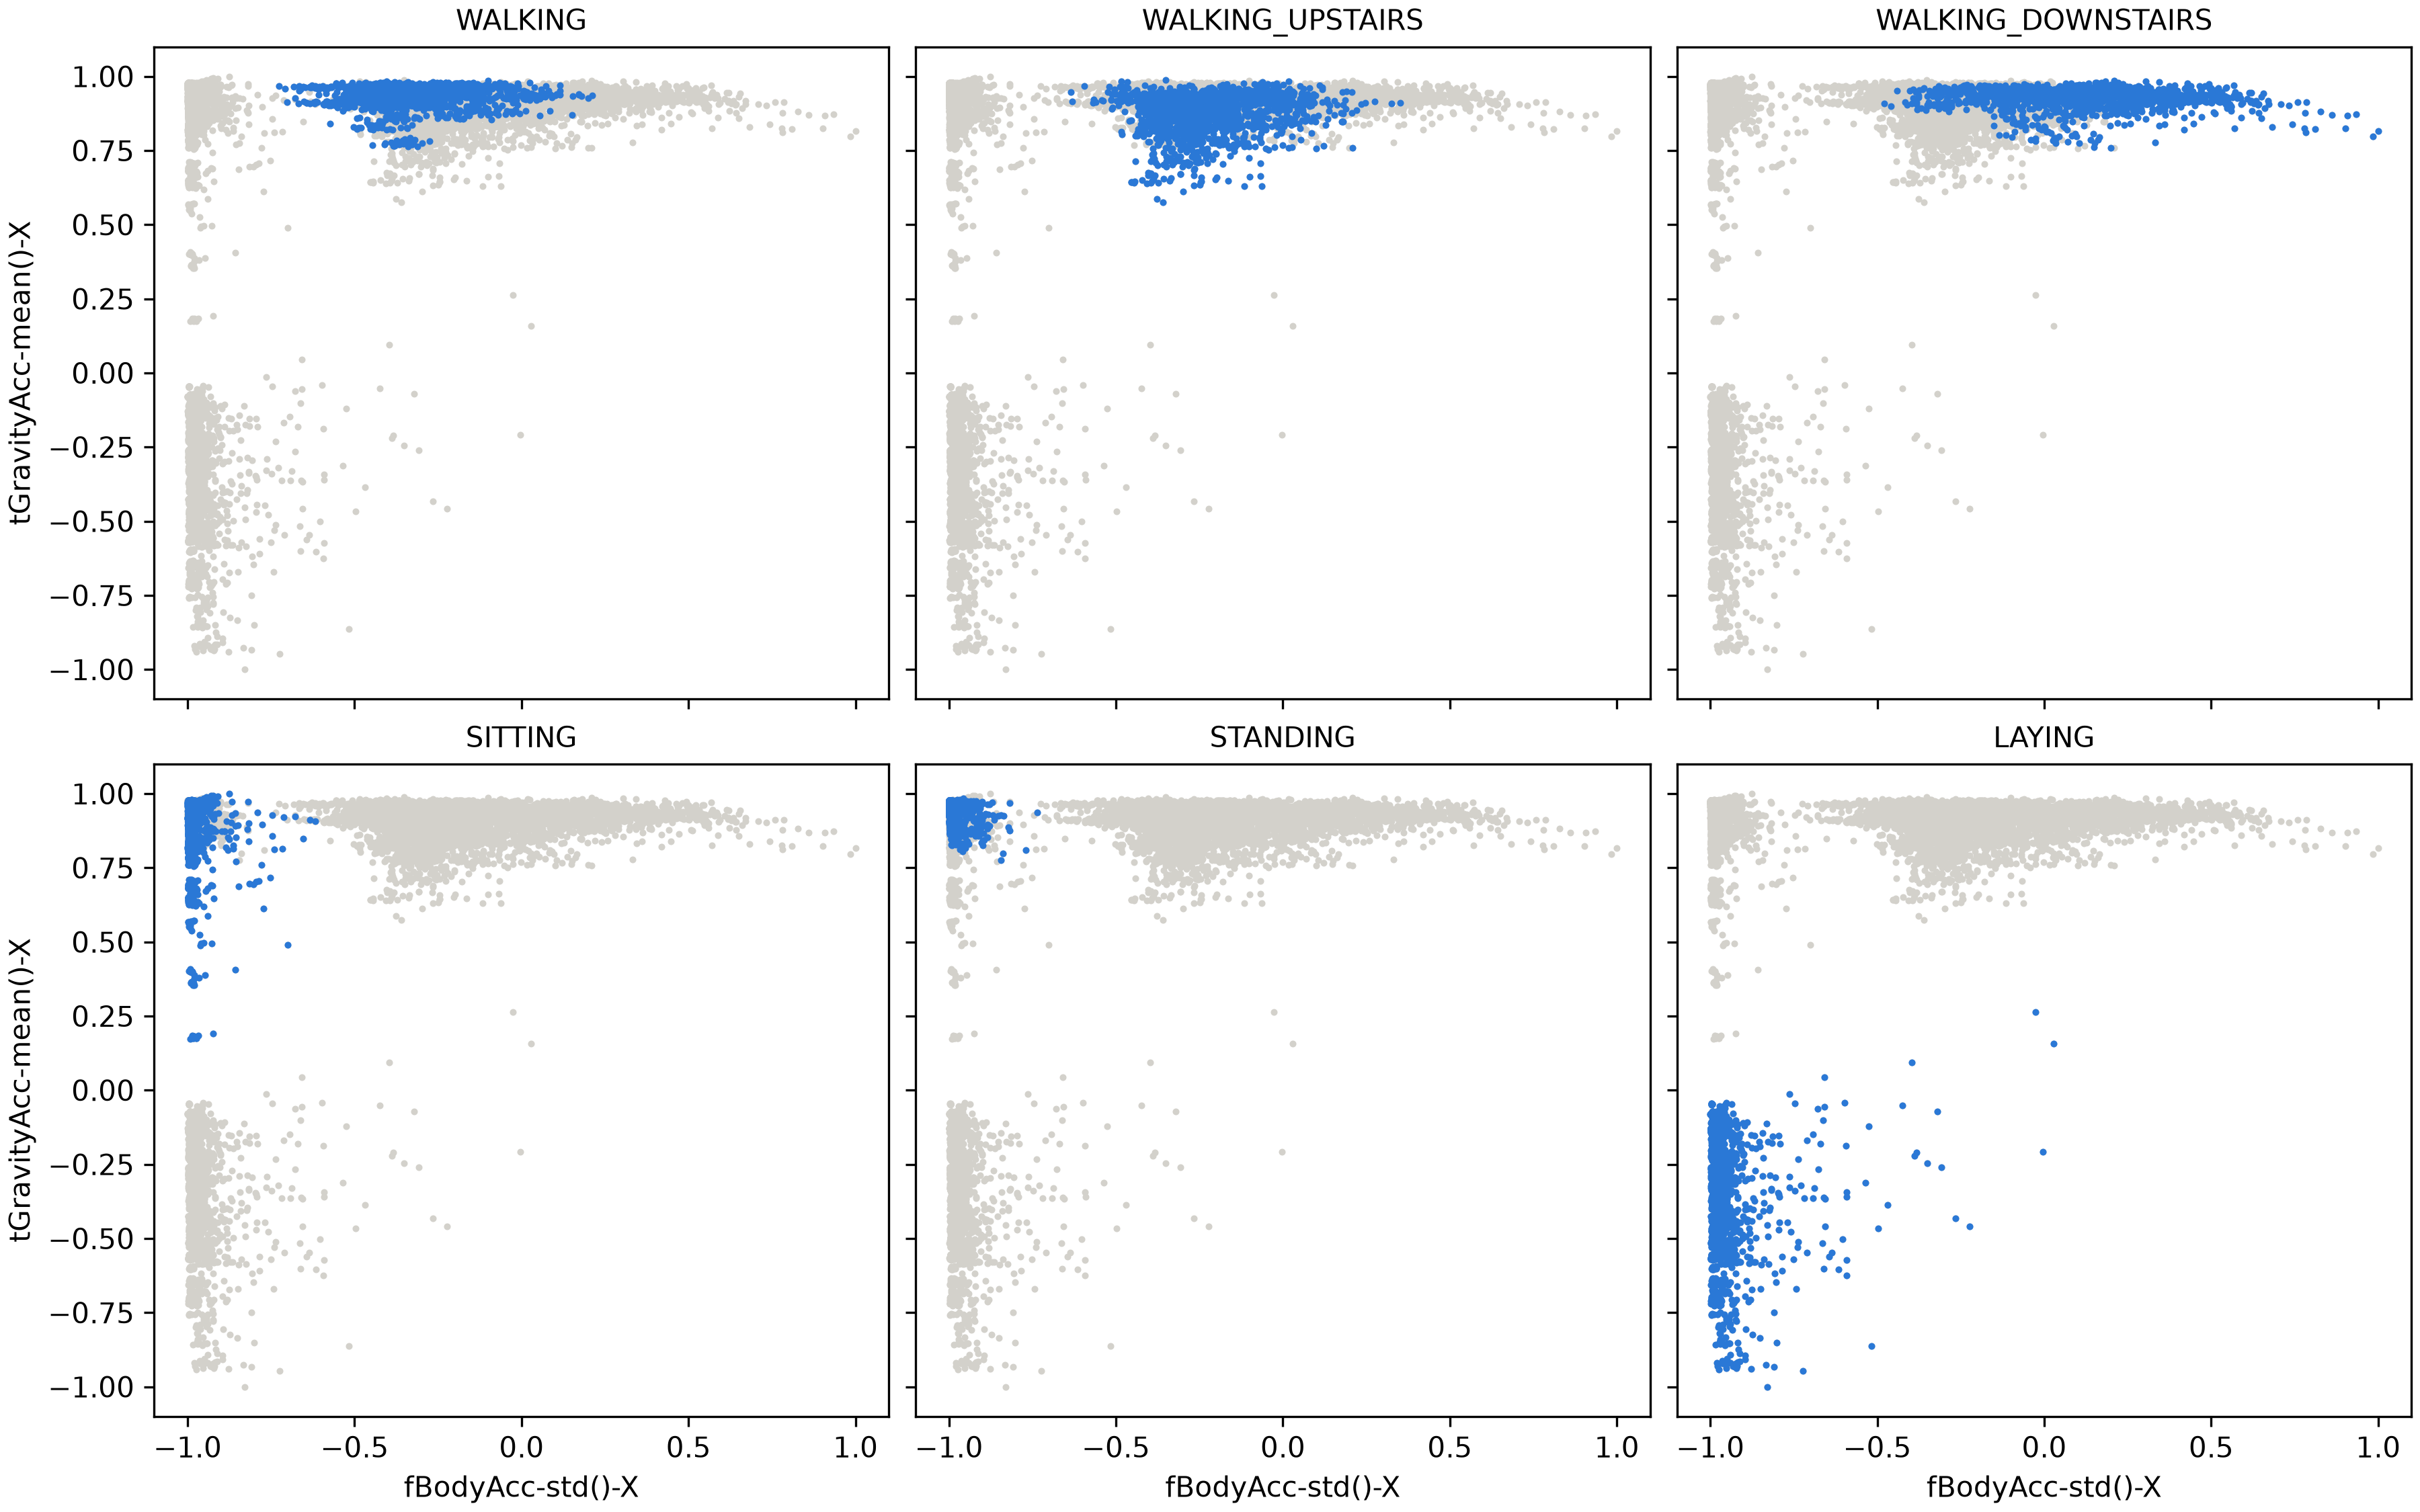
\includegraphics[width=0.85\textwidth]{figures/two_features.png}
\caption{\texttt{fBodyAcc-std()-X} vs.\ \texttt{tGravityAcc-mean()-X}.}
\label{fig:twofeatures}
\end{figure}

\begin{figure}[htbp]
\centering
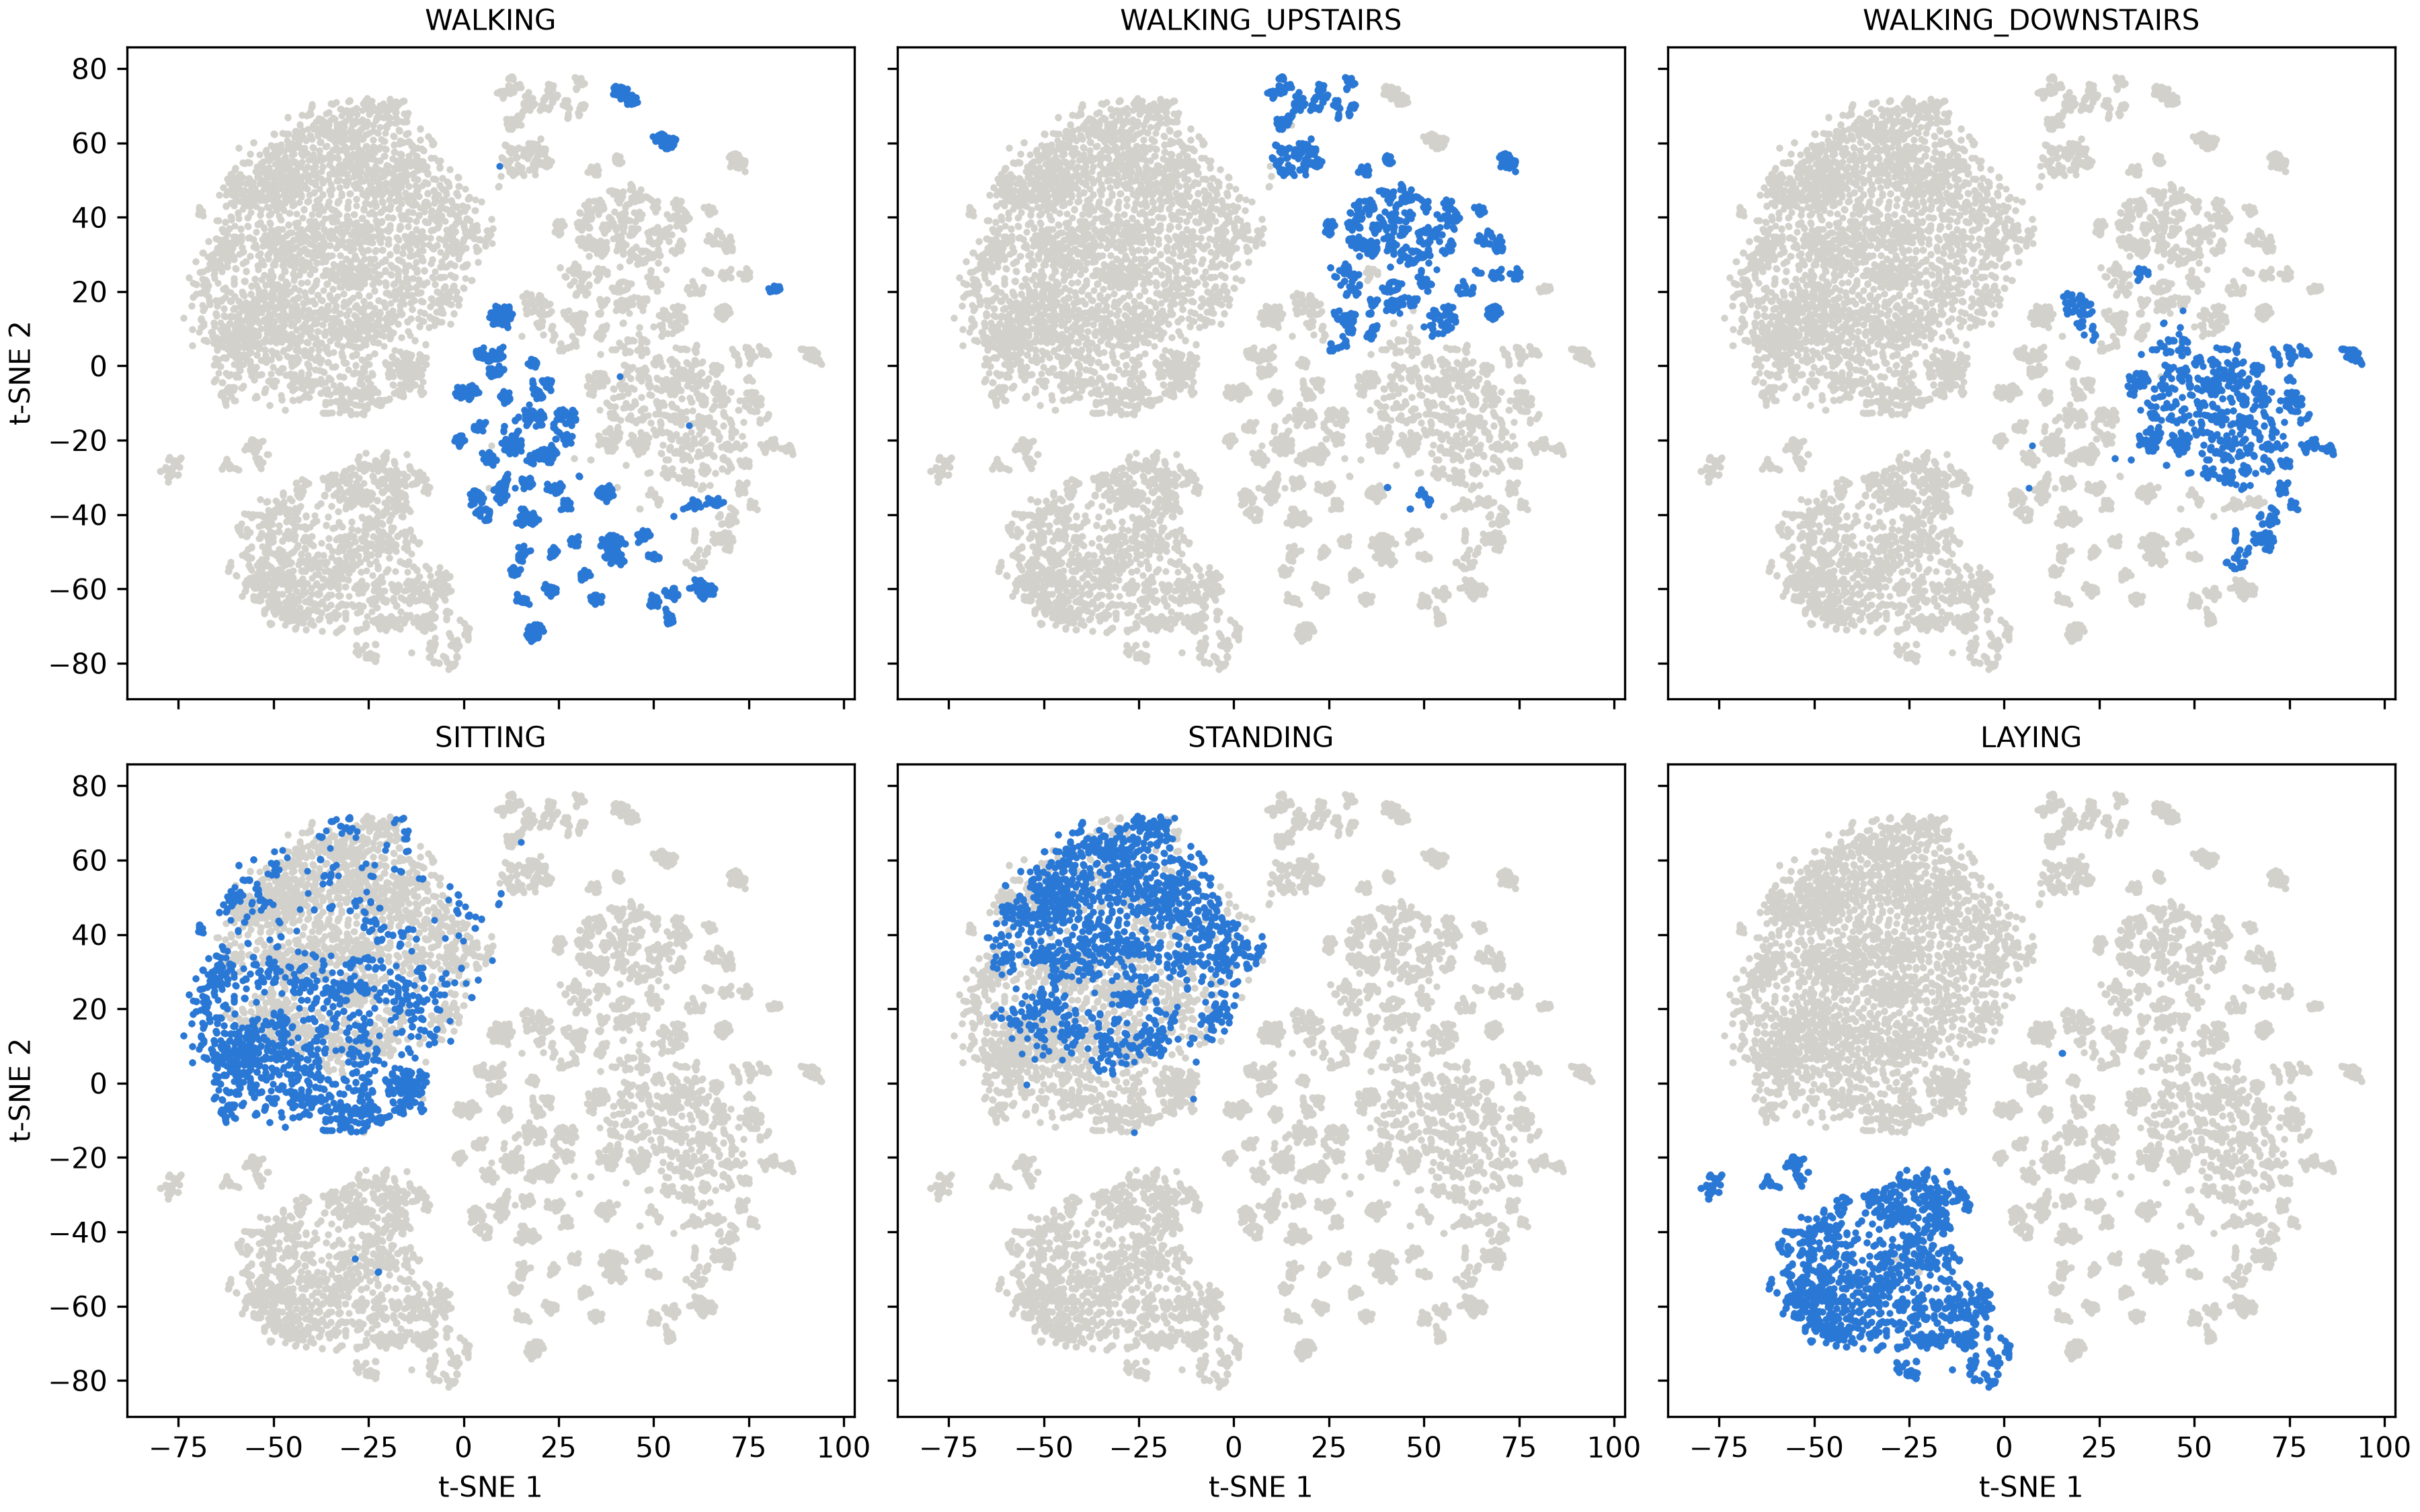
\includegraphics[width=0.85\textwidth]{figures/tsne.png}
\caption{t-SNE embedding of the 540 distinct features; the axes have no meaning.}
\label{fig:tsne}
\end{figure}

Interpretation:
\begin{itemize}
  \item PCA, \autoref{fig:pca}: PC1 $= 60.8\%$, PC2 $= 4.8\%$ of the variance.
  \begin{itemize}
    \item PC1 separates the static from the dynamic activities into two groups.
    \item Within each group, the activities overlap.
  \end{itemize}
  \item Two features, \autoref{fig:twofeatures}:
  \begin{itemize}
    \item \feat{fBodyAcc-std()-X} separates the static from the dynamic activities: mean $\in [-0.99, -0.96]$ vs.\ $[-0.32, 0.12]$.
    \item \feat{tGravityAcc-mean()-X} separates \feat{LAYING}: mean $= -0.375$ vs.\ $[0.875, 0.941]$ for the other activities.
    \item Sitting and standing overlap.
  \end{itemize}
  \item t-SNE, \autoref{fig:tsne}:
  \begin{itemize}
    \item Laying, the walking activities and the other static activities form distinct regions.
    \item Sitting and standing share one region, partly separated.
    \item Walking splits into many small, tight clusters.
    \item Laying is the most distinguishable group.
  \end{itemize}
\end{itemize}

\FloatBarrier
\bibliographystyle{alpha}
\bibliography{biblio}

\end{document}
